% $Header$
% MBDyn (C) is a multibody analysis code.
% http://www.mbdyn.org
%
% Copyright (C) 1996-2010
%
% Pierangelo Masarati  <masarati@aero.polimi.it>
%
% Dipartimento di Ingegneria Aerospaziale - Politecnico di Milano
% via La Masa, 34 - 20156 Milano, Italy
% http://www.aero.polimi.it
%
% Changing this copyright notice is forbidden.
%
% This program is free software; you can redistribute it and/or modify
% it under the terms of the GNU General Public License as published by
% the Free Software Foundation (version 2 of the License).
% 
%
% This program is distributed in the hope that it will be useful,
% but WITHOUT ANY WARRANTY; without even the implied warranty of
% MERCHANTABILITY or FITNESS FOR A PARTICULAR PURPOSE.  See the
% GNU General Public License for more details.
%
% You should have received a copy of the GNU General Public License
% along with this program; if not, write to the Free Software
% Foundation, Inc., 59 Temple Place, Suite 330, Boston, MA  02111-1307  USA

\chapter{General}\label{sec:GENERAL}
This chapter describes how data structures are read 
and how they participate, as building blocks, to the definition
of specific cards.
Consistency across the software and the input file has been 
a driving principle in designing the input of MBDyn.
As such, the very same elementary data structures are present
in very different contexts.



\section{Types}



\subsection{Keywords}
In MBDyn's input a lot of so-called ``keywords'' appear literarly
in the input file.
They are case-insensitive and may have an arbitrary amount of space
in between.
For example, `\kw{control data}', `\kw{Control Data}',
and `\kw{controldata}' are equivalent.

However, most of the keywords are context-dependent,
so they are not illustrated altogether in a dedicated section,
but rather presented in relation to the contexts they may appear in.




\subsection{Strings}
Literal strings are not used very much in MBDyn.
However, they may be used in quite a few significant places,
for example to indicate file names, so few details on their syntax
are provided.

Strings are typically delimited by double quotes (`\texttt{"}').
When a string is expected, the parser looks for the opening 
double quotes and eats up all the white space before it.
Then all characters are read as they are until the closing 
double quotes are encountered.
The escape character is the backslash (`$\backslash$'); it is used:
\begin{itemize}
	\item to escape the escape character itself (`$\backslash$');
	\item to escape any double quotes that are part of the string,
		and would otherwise be interpreted as the closure
		of the string;
	\item to break a string on multiple lines by placing it
		before the newline character (`\texttt{$\backslash$n}');
		in this case, the escape character and the newline
		are eaten up;
	\item to allow the use of non-printing characters,
		represented in the form `\texttt{$\backslash$<hexpair>}',
		so that the hexadecimal representation of the
		non-printing char is converted into its integer
		equivalent in the 0--255 range.
\end{itemize}
Character sets different from ASCII are not supported.



\subsection{Numeric Values}
Every time a numeric value is expected, the result of evaluating 
a mathematical expression can be used, including variable declaration 
and assignment (variable names and values are kept in memory throughout
the input phase and the simulation) and simple math functions.
Named variables and non-named constants are strongly typed; three types are
currently available, \kw{integer}, \kw{real}, and \kw{string}.

Operations are strongly typed and perform implicit cast when allowed.
For instance \texttt{1+2.5} returns a \kw{real} whose value 
is \texttt{3.5}, since one of the 
two addenda is \kw{real}, while \texttt{1/3} returns \texttt{0} because 
both types are implicit integers and the integer division is used.

An empty field, delimited by a valid separator (a comma or a semicolon,
depending on whether other arguments are expected or not) returns the
(program supplied) default value for that field, if supplied by the caller, 
otherwise the parser automatically defaults to zero.

Multiple expressions can be used, provided they are enclosed in plain 
brackets and are separated by semicolons; the result 
of the last expression will be used as the expected numeric value,
but all the expressions (which may have persistent effects, 
like variable declarations and assignments) will be evaluated.

\paragraph{Example.} \
\begin{verbatim}
    1.                                                     # == 1.
    (real r = 2.*pi; integer i = 3; sin(i*r*Time+.87))     # == sin(6*pi*Time+.87)
\end{verbatim}
The latter sequence evaluates to $ \sin\plbr{6\pi{t}+.87} $,
depending on the current value of the pre-defined variable \kw{Time}.
The constant \kw{pi} is always defined as $ \pi $ with machine precision
(the macro \texttt{M\_PI} in the standard C header file \texttt{math.h}).
Other constants are pre-defined, as illustrated
in Table~\ref{tab:MATHP-VARS}.

When MBDyn is invoked with the `\texttt{-H}' option,
\begin{verbatim}
    mbdyn -H
\end{verbatim}
it prints the predefined variables table.
A typical output is shown in Figure~\ref{fig:MBDYN-H}.
Values are stored with the maximum precision allowed by the underlying
\kw{real} type (by default, double precision, 64 bit).

\begin{figure}
\label{fig:MBDYN-H}
\centering
\small
\begin{minipage}{120mm}
\begin{verbatim}
user@host:~> mbdyn -H

MBDyn - MultiBody Dynamics 1.2-Engineering
compiled on May 20 2004 at 10:42:24

Copyright 1997-2010 (C) Paolo Mantegazza and Pierangelo Masarati,
Dipartimento di Ingegneria Aerospaziale, Politecnico di Milano.

MBDyn is free software, covered by the GNU General Public License, and you are
welcome to change it and/or distribute copies of it under certain conditions.
Use 'mbdyn --license' to see the conditions.
There is absolutely no warranty for MBDyn.  Use "mbdyn --warranty" for details.

default symbol table:
  real mm2in = 0.0393701
  real lb2kg = 0.4535
  real m2in = 39.3701
  real m2ft = 3.28084
  real in2m = 0.0254
  real in2mm = 25.4
  real pi = 3.14159
  real deg2rad = 0.0174533
  real kg2lb = 2.20507
  real e = 2.71828
  real rad2deg = 57.2958
  int RAND_MAX = 2147483647
  real ft2m = 0.3048

MBDyn terminated normally
user@host:~>
\end{verbatim}
\end{minipage}
\caption{Predefined variables in math parser}
\end{figure}

The variable \kw{Time} is declared, defined and initialized\footnote{
    A variable is \emph{declared} when its name enters the namespace;
    it is \emph{defined} when it can be referenced;
    it is \emph{initialized} when it is first assigned a value
} from the beginning of the control data section, and during the solution 
phase it is assigned the value of the current time. 

Table~\ref{tab:MATHP-OPERATORS} shows the supported mathematical 
operators, while Table~\ref{tab:MATHP-FUNCTIONS} shows the built-in
mathematical functions.
The supported types are listed in Table~\ref{tab:MATHP-TYPES}.
Table~\ref{tab:MATHP-VARS} lists the predefined variables; notice
that they're treated exactly as user-defined variables, so they 
can be reassigned.

\begin{table}
	\begin{center}
	\caption{Built-in mathematical operators in math parser
	(from higher to lower precedence)}\label{tab:MATHP-OPERATORS}
	\begin{tabular}{lll}
		\hline
		\multicolumn{1}{c}{\textbf{Operator}} & 
		\multicolumn{1}{c}{\textbf{Type}} &
		\multicolumn{1}{c}{\textbf{Description}} \\
		\hline
		\texttt{\^} & Binary, right & Power \\
		\texttt{+} & Unary, left & Plus sign \\
		\texttt{-} & Unary, left & Minus sign \\
		\texttt{*} & Binary, left & Multiplication \\
		\texttt{/} & Binary, left & Division \\
		\texttt{+} & Binary, left & Addition \\
		\texttt{-} & Binary, left & Subtraction \\
		\texttt{>} & Binary, left & Greater than \\
		\texttt{>=} & Binary, left & Greater than or equal to \\
		\texttt{==} & Binary, left & Equal to \\
		\texttt{<=} & Binary, left & Less than or equal to \\
		\texttt{<} & Binary, left & Less than \\
		\texttt{!=} & Binary, left & Not equal \\
		\texttt{!} & Unary, right & NOT \\
		\texttt{\&\&} & Binary, left & AND \\
		\texttt{||} & Binary, left & OR \\
		\texttt{\~{}|} & Binary, left & XOR (exclusive OR) \\
		\texttt{=} & Binary, right & Assignment \\
		\hline
	\end{tabular}
	\end{center}
	\footnotesize
	Note: ``left'' and ``right'' refer to the associativity
	of the operators. \\
	Note: the \kw{string} type only supports the binary ``+'' operator.
\end{table}

\begin{table}
	\begin{center}
	\caption{Built-in mathematical functions 
		in math parser}\label{tab:MATHP-FUNCTIONS}
	\begin{tabular}{llll}
		\hline
		\multicolumn{1}{c}{\textbf{Name}} &
		\multicolumn{1}{c}{\textbf{Returns}} &
		\multicolumn{1}{c}{\textbf{Arg[s]}} &
		\multicolumn{1}{c}{\textbf{Description}} \\
		\hline
		\kw{asin}	& Real		& Real		& Arc sine \\
		\kw{acos}	& Real		& Real		& Arc cosine \\
		\kw{atan}	& Real		& Real		& Arc tangent \\
		\kw{actan}	& Real		& Real		& Arc co-tangent \\
		\kw{atan2}	& Real		& Real, Real	& (Robust) arc tangent \\
		\kw{actan2}	& Real		& Real, Real	& (Robust) arc co-tangent \\
		\kw{cos}	& Real		& Real		& Cosine \\
		\kw{sin}	& Real		& Real		& Sine \\
		\kw{tan}	& Real		& Real		& Tangent \\
		\kw{ctan}	& Real		& Real		& Co-tangent \\
		\kw{cosh}	& Real		& Real		& Hyperbolic cosine \\
		\kw{sinh}	& Real		& Real		& Hyperbolic sine \\
		\kw{tanh}	& Real		& Real		& Hyperbolic tangent \\
		\kw{ctanh}	& Real		& Real		& Hyperbolic co-tangent \\
		\kw{acosh}	& Real		& Real		& Hyperbolic arc cosine \\
		\kw{asinh}	& Real		& Real		& Hyperbolic arc sine \\
		\kw{atanh}	& Real		& Real		& Hyperbolic arc tangent \\
		\kw{actanh}	& Real		& Real		& Hyperbolic arc co-tangent \\
		\kw{exp}	& Real		& Real		& Exponential \\
		\kw{log}	& Real		& Real		& Natural logarithm \\
		\kw{log10}	& Real		& Real		& Base 10 logarithm \\
		\kw{sqrt}	& Real		& Real		& Square root \\
		\kw{abs}	& Real		& Real		& Absolute value \\
		\kw{sign}	& Real		& Real		& Sign \\
		\kw{copysign}	& Real		& Real, Real	& First arg with sign of second \\
		\kw{floor}	& Integer	& Real		& Closest integer from below \\
		\kw{ceil}	& Integer	& Real		& Closest integer from above \\
		\kw{round}	& Integer	& Real		& Closest integer \\
		\kw{rand}	& Integer	& Void		& random integer 
			$\sqbr{0,\mathrm{RAND\_MAX}}$ \\
		\kw{random}	& Real		& Void		& random real $\sqbr{-1.0,1.0}$ \\
		\kw{seed}	& Void		& Integer	& Seeds the random number generator \\
		\kw{step}	& Real		& Real		& Step function \\
		\kw{ramp}	& Real		& Real		& Ramp function \\
		\kw{sramp}	& Real		& Real, Real	& Saturated ramp function \\
		\kw{par}	& Real		& Real		& Parabolic function \\
		\kw{print}	& Void		& Real		& Prints a value to standard output \\
		\hline
	\end{tabular}
	\end{center}
\end{table}

\begin{table}
	\begin{center}
	\caption{Built-in types in math parser}\label{tab:MATHP-TYPES}
	\begin{tabular}{ll}
		\hline
		\multicolumn{1}{c}{\textbf{Name}} &
		\multicolumn{1}{c}{\textbf{Description}} \\
		\hline
		\kw{bool} & Boolean number (promoted to \kw{integer}, \kw{real},
			or \kw{string} (0 or 1), whenever required) \\
		\kw{integer} & Integer number (promoted to \kw{real}, or \kw{string},
			whenever required) \\
		\kw{real} & Real number (promoted to \kw{string}
			whenever required) \\
		\kw{string} & Text string \\
		\hline
	\end{tabular}
	\end{center}
\end{table}

\begin{table}
	\begin{center}
	\caption{Predefined variables in math parser}\label{tab:MATHP-VARS}
	\begin{tabular}{lll}
		\hline
		\multicolumn{1}{c}{\textbf{Name}} &
		\multicolumn{1}{c}{\textbf{Type}} &
		\multicolumn{1}{c}{\textbf{Value}} \\
		\hline
		\kw{Time} & Real & Current simulation time \\
		\kw{TimeStep} & Real & Current simulation time step \\
		\kw{Step} & Integer & Current simulation step \\
		\kw{Var} & Real & \multicolumn{1}{p{.5\textwidth}}{Set
			by dof, node, or element drive caller with
			DOF value, node or element private data value} \\
		\\
		\kw{e} & Real & Neper's number \\
		\kw{pi} & Real & $\pi$ \\
		\kw{RAND\_MAX} & Integer & Maximum random integer \\
		\\
		\kw{in2m} & Real & Inch to meter ratio (0.0254) \\
		\kw{m2in} & Real & Meter to inch ratio (1.0/0.0254) \\
		\kw{in2mm} & Real & Inch to meter ratio (25.4) \\
		\kw{mm2in} & Real & Meter to inch ratio (1.0/25.4) \\
		\kw{ft2m} & Real & Foot to meter ratio (0.3048) \\
		\kw{m2ft} & Real & Meter to foot ratio (1.0/0.3048) \\
		\kw{lb2kg} & Real & Pound to kilogram ratio (0.4535) \\
		\kw{kg2lb} & Real & Kilogram to pound ratio (1.0/0.4535) \\
		\kw{deg2rad} & Real & Degree to radian ratio ($\pi$/180) \\
		\kw{rad2deg} & Real & Radian to degree ratio (180/$\pi$) \\
		\hline
	\end{tabular}
	\end{center}
\end{table}

\subsection{Namespaces}
\label{sec:GENERAL:NAMESPACE}
The math parser uses the notion of \emph{namespace} to separate
functions.
The functions listed in Table~\ref{tab:MATHP-FUNCTIONS}
are implicitly defined in the \kw{default} namespace, 
i.e.\ they should be referenced by writing
\begin{verbatim}
    default::sqrt(2.)
\end{verbatim}
Other namespaces may be defined by the user, and loaded by means
of the \kw{module load} card described
in Section~\ref{sec:GENERAL:MODULE-LOAD}.

The namespace that refers to the current model is loaded by default.
Its name is \kw{model}, and contains the functions 
defined in Table~\ref{tab:MODEL-NS-FUNCS}.

\begin{table}
	\begin{center}
	\caption{Functions in the \kw{model} namespace}
	\label{tab:MODEL-NS-FUNCS}
	\begin{tabular}{lllp{.6\textwidth}}
		\hline
		\multicolumn{1}{c}{\textbf{Name}} &
		\multicolumn{1}{c}{\textbf{Ret.}} &
		\multicolumn{1}{c}{\textbf{Arg[s]}} &
		\multicolumn{1}{c}{\textbf{Description}} \\
		\hline
		\kw{position}	& Real	& Integer		& norm of structural node position \\
		\kw{position2}	& Real	& Integer		& square norm of structural node position \\
		\kw{xposition}	& Real	& Integer		& $X$ component of structural node position \\
		\kw{yposition}	& Real	& Integer		& $Y$ component of structural node position \\
		\kw{zposition}	& Real	& Integer		& $Z$ component of structural node position \\
		\kw{distance}	& Real	& Integer, Integer	& distance between structural nodes \\
		\kw{distance2}	& Real	& Integer, Integer	& square distance between structural nodes \\
		\kw{xdistance}	& Real	& Integer, Integer	& $X$ component of distance between structural nodes \\
		\kw{ydistance}	& Real	& Integer, Integer	& $Y$ component of distance between structural nodes \\
		\kw{zdistance}	& Real	& Integer, Integer	& $Z$ component of distance between structural nodes \\
		\kw{xunitvec}	& Real	& Integer, Integer	& $X$ component of unit vector between structural nodes \\
		\kw{yunitvec}	& Real	& Integer, Integer	& $Y$ component of unit vector between structural nodes \\
		\kw{zunitvec}	& Real	& Integer, Integer	& $Z$ component of unit vector between structural nodes \\
		\kw{anglerel}	& Real	& Integer, Integer	& angle between structural nodes (norm of angular vector) \\
		\kw{xanglerel}	& Real	& Integer, Integer	& $X$ component of angular vector between structural nodes \\
		\kw{yanglerel}	& Real	& Integer, Integer	& $Y$ component of angular vector between structural nodes \\
		\kw{zanglerel}	& Real	& Integer, Integer	& $Z$ component of angular vector between structural nodes \\
		\kw{velocity}	& Real	& Integer		& norm of structural node velocity \\
		\kw{velocity2}	& Real	& Integer		& square norm of structural node velocity \\
		\kw{xvelocity}	& Real	& Integer		& $X$ component of structural node velocity \\
		\kw{yvelocity}	& Real	& Integer		& $Y$ component of structural node velocity \\
		\kw{zvelocity}	& Real	& Integer		& $Z$ component of structural node velocity \\
		\kw{vrel}	& Real	& Integer, Integer	& norm of relative velocity between structural nodes \\
		\kw{vrel2}	& Real	& Integer, Integer	&
				square norm of relative velocity between structural nodes \\
		\kw{xvrel}	& Real	& Integer, Integer	&
				$X$ component of relative velocity between structural nodes \\
		\kw{yvrel}	& Real	& Integer, Integer	&
				$Y$ component of relative velocity between structural nodes \\
		\kw{zvrel}	& Real	& Integer, Integer	&
				$Z$ component of relative velocity between structural nodes \\
		\kw{drive}	& Real	& Integer, Real		&
				evaluates the \htmlref{\kw{drive caller}}{sec:DRIVE-CALLER}
				indicated by its label (the first argument)
				for the input specified as second argument \\
		\kw{sf}\texttt{::}\bnt{name}	& Real	& Real			&
				evaluates the \htmlref{\kw{scalar function}}{sec:SCALARFUNCS}
				\nt{name} for the input specified as argument \\
		\hline
	\end{tabular}
	\end{center}
\end{table}


\subsection{Plugin Variables}
\label{sec:GENERAL:PLUGIN}
Plugin variables, or plugins, as the name states, are pluggable extensions
to the math parser that allow to register mechanisms to bind a variable
to some means to dynamically generate its value.
As a consequence, any time a variable declared as part of a plugin
is used, its value is dynamically evaluated executing the related code.

There are built-in plugins that allow to link variables to the value
of degrees of freedom and to special parameters computed by nodes
and elements.

The syntax of a plugin consists in specially defining a variable
so that it gets registered to the appropriate code:
%\begin{verbatim}
\begin{Verbatim}[commandchars=\\\{\}]
    \kw{set} : OSQBR \bnt{plugin} , \bnt{var} [ , \bnt{arglist} ] CSQBR ;
    \bnt{arglist} ::= \bnt{arg} [ , ... ]
\end{Verbatim}
%\end{verbatim}
where \texttt{OSQBR} and \texttt{CSQBR} stand for `open' and `close'
square brackets, respectively, which shouldn't be confused with those
that indicate optional parameters.

In the following, the built-in plugins\footnote{Built-in and plug-in
may sound contradictory, and in fact they are.  However, consider
that the mathematical parser is essentially independent of MBDyn
(in fact, it has been turned into a command-line calculator
in \texttt{cl(1)}), so, from this point of view, built-in plug-ins
are used to plug MBDyn information into an independent, lower-level
piece of code.} are illustrated.
For details on nodes, elements, their properties and the information
they can expose, see the related sections.

\subsubsection{Dof plugin}
\emph{Note: this plugin is now obsoleted by the \kw{node} plugin,
which allows to access more significant information about nodes,
including the value of the degrees of freedom.}

The \kw{dof} plugin allows to link a variable to a specific degree of freedom
of a node, or to its derivative, whenever defined.
The syntax is
%\begin{verbatim}
\begin{Verbatim}[commandchars=\\\{\}]
    \bnt{plugin} ::= \kw{dof}
    \bnt{arglist} ::= \bnt{label} , \bnt{type} [ , \bnt{index} ] , \{ \kw{algebraic} | \kw{differential} \}
\end{Verbatim}
%\end{verbatim}
where
\nt{label} is the label of the node,
\nt{type} is the node type,
\nt{index} is the index of the degree of freedom that is requested,
if the node has more than one, while
\kw{algebraic} and \kw{differential} refer to the value of the dof
and of its derivative, respectively.
The derivative can be requested only for those degrees of freedom
that have one.

\paragraph{Example.} \
The variable \texttt{VARNAME} takes the value of the derivative
of \kw{abstract} node \texttt{NODENAME}
\begin{verbatim}
    set: integer NODENAME = 1000;
    # the node must exist
    set: [dof,VARNAME,NODENAME,abstract,differential];
\end{verbatim}



\subsubsection{Node plugin}
The \kw{node} plugin allows to link a variable to any data a node
can expose, including the values of its degrees of freedom.
The syntax is
%\begin{verbatim}
\begin{Verbatim}[commandchars=\\\{\}]
    \bnt{plugin} ::= \kw{node}
    \bnt{arglist} ::= \bnt{label} , \bnt{type}
        [ , \{ [ \kw{index=} ] \bnt{index} | \kw{string=} \bnt{name} \} ]
\end{Verbatim}
%\end{verbatim}
where
\nt{label} is the label of the node,
\nt{type} is the node type,
and the mutually exclusive \nt{index} and \nt{name} represent the index
of the datum that is requested, \nt{name} being a user-friendly
representation of the actual index.
The \nt{index} form is the default; however, the \nt{name} form is recommended.
Note that \nt{name} should be enclosed in double quotes,
although not strictly required.
In fact, some node types allow data names that include square brackets.
In those cases, double-quote enclosing is needed to avoid parsing errors,
since closing square brackets indicate the end
of the plugin variable specification.

\paragraph{Example.} \
This implements the same variable defined in the \kw{dof} example,
where the variable \texttt{VARNAME} takes the value of the derivative
of \kw{abstract} node \texttt{NODENAME}
\begin{verbatim}
    set: integer NODENAME = 1000;
    # the node must exist
    set: [node,VARNAME,NODENAME,abstract,string,"xP"];
\end{verbatim}



\subsubsection{Element plugin}
The \kw{element} plugin allows to link a variable to any data an element
can expose, including the values of its degrees of freedom.
The syntax is
%\begin{verbatim}
\begin{Verbatim}[commandchars=\\\{\}]
    \bnt{plugin} ::= \kw{element}
    \bnt{arglist} ::= \bnt{label} , \bnt{type}
        [ , \{ [ \kw{index=} ] \bnt{index} | \kw{string=} \bnt{name} \} ]
\end{Verbatim}
%\end{verbatim}
where
\nt{label} is the label of the element,
\nt{type} is the element type,
and the mutually exclusive \nt{index} and \nt{name} represent the index
of the datum that is requested, \nt{name} being a user-friendly
representation of the actual index.
The \nt{index} form is the default; however, the \nt{name} form is recommended.
Note that \nt{name} should be enclosed in double quotes,
although not strictly required.
In fact, some element types allow names that include square brackets.
In those cases, double-quote enclosing is needed to avoid parsing errors,
since closing square brackets indicate the end
of the plugin variable specification.

\paragraph{Example.} \
The variable \texttt{VARNAME} takes the value of the $z$ component 
of the reaction force of \kw{joint} \texttt{ELEMNAME}
\begin{verbatim}
    set: integer ELEMNAME = 1000;
    # the joint must exist
    set: [element,VARNAME,ELEMNAME,joint,string,"Fz"];
\end{verbatim}



\section{Higher-Order Math Structures}
Every time a higher-order mathematical structure is expected, it can be
preceded by a keyword that influences how the structure is read.
All of the available structures support the keyword \kw{null}
which causes the structure to be initialized with zeros.
When a non-null value is input, it can be followed by the keyword
\kw{scale} with a scale factor; the scale factor can be any
mathematical expression.
This is useful to rescale structure values by reassigning the value 
of the scale factor.
The main data structures are:
\subsection{$3 \times 1$ vectors}
\begin{enumerate}
    \item general case: a sequence of 3 reals, comma-separated.
    \item null vector: keyword \kw{null}; the vector is initialized
	with zeros.
\end{enumerate}
As an example, all the following lines define an empty $3 \times 1$ vector:
\begin{verbatim}
    default
    null
    0.,0.,0.
    ,,
\end{verbatim}
the first case is correct if no default was actually available
for that specific vector, thus falling back to three zeros.
The following rescales an arbitrary vector
\begin{verbatim}
    cos(pi/3.),0.,sin(pi/3.), scale, 100.
\end{verbatim}

\subsection{$6 \times 1$ vectors}
\begin{enumerate}
    \item general case: a sequence of 6 reals, comma-separated.
    \item null vector: keyword \kw{null}; the vector is initialized 
    with zeros.	
\end{enumerate}
\subsection{$3 \times 3$ matrices}
\begin{enumerate}
    \item general case: a sequence of 9 reals, comma-separated, which
    represent the row-oriented coefficients $ a_{11} $, $ a_{12}$ ,
    \ldots, $ a_{32} $, $ a_{33} $.
    \emph{Note: the 9 coefficients can be preceded by the keyword
    \kw{matr} for consistency with other entities; its use is recommended
    whenever an ambiguity is possible.}
\begin{equation}
	\T{m} = \sqbr{\matr{ccc}{
		a_{11} & a_{12} & a_{13} \\
		a_{21} & a_{22} & a_{23} \\
		a_{31} & a_{32} & a_{33}
	}}
\end{equation}
    \item symmetric matrix: keyword \kw{sym}, followed by a sequence
    of 6 reals, comma-separated, that represents the upper triangle, 
    row-oriented coefficients of a symmetric matrix, 
    e.g. $ a_{11} $, \ldots , $ a_{13} $, $ a_{22} $, $ a_{23} $, $ a_{33} $.
\begin{equation}
	\T{m} = \sqbr{\matr{ccc}{
		a_{11} & a_{12} & a_{13} \\
		a_{12} & a_{22} & a_{23} \\
		a_{13} & a_{23} & a_{33}
	}}
\end{equation}
    \item skew symmetric matrix: keyword \kw{skew}, followed by a sequence
    of 3 reals, comma-separated, that are the components of the vector $\T{v}$
    that generates a skew symmetric matrix $\T{m}=\T{v}\times{}$:
\begin{equation}
	\T{m} = \sqbr{\matr{ccc}{
		0 & -v_3 & v_2 \\
		v_3 & 0 & -v_1 \\
		-v_2 & v_1 & 0
	}}
\end{equation}
    \item diagonal matrix: keyword \kw{diag}, followed by a sequence
    of 3 reals, comma-separated, that represent the diagonal coefficients 
    of a diagonal matrix, namely $a_{11}$, $a_{22}$, $a_{33}$
\begin{equation}
	\T{m} = \sqbr{\matr{ccc}{
		a_{11} & 0 & 0 \\
		0 & a_{22} & 0 \\
		0 & 0 & a_{33}
	}}
\end{equation}
    \item identity matrix: keyword \kw{eye}; the matrix is initialized
    as the identity matrix, that is a null matrix except for the diagonal 
    coefficients that are 1.
    \item null matrix: keyword \kw{null}; the matrix is initialized 
    with zeros.
\end{enumerate}
For example, the identity matrix can be defined as:
\begin{verbatim}
    matr, 1.,0.,0.,  0.,1.,0.,  0.,0.,1.
    1.,0.,0.,  0.,1.,0.,  0.,0.,1.        # ``matr'' omitted
    sym, 1.,0.,0.,  1.,0.,  1.            # upper triangular part
    diag, 1.,1.,1.                        # diagonal
    eye                                   # a la matlab
\end{verbatim}
Although not required, for better readability it is recommended to format
the above data as
\begin{verbatim}
    matr,
        1.,0.,0.,
        0.,1.,0.,
        0.,0.,1.
    1.,0.,0.,
    0.,1.,0.,
    0.,0.,1.                              # ``matr'' omitted
    sym,
        1.,0.,0.,
           1.,0.,
              1.                          # upper triangular part
    diag, 1.,1.,1.                        # diagonal
    eye                                   # a la matlab
\end{verbatim}

\begin{figure}
\centering
\psfrag{a}{(a)}
\psfrag{b}{(b)}
\psfrag{c}{(c)}
\psfrag{d}{(d)}
\psfrag{1}{1}
\psfrag{2}{2}
\psfrag{2b}{2'}
\psfrag{3}{3}
\psfrag{1c}{\fbox{1}}
\psfrag{2c}{\fbox{2}}
\psfrag{2bc}{\fbox{2'}}
\psfrag{3c}{\fbox{3}}
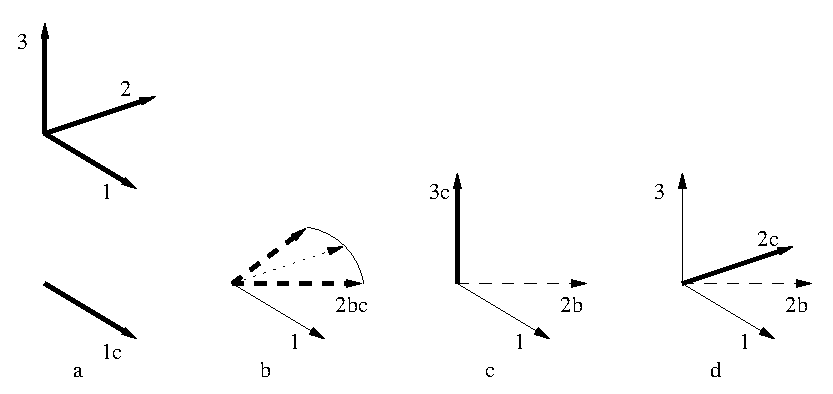
\includegraphics[width=.9\textwidth]{MatR2vec}
\caption{Construction of $3 \times 3$ orientation matrix from two
non-parallel vectors.}
\label{fig:general:orientation-matrices:MatR2vec}
\end{figure}

\subsection{$3 \times 3$ orientation matrices}
\begin{enumerate}
\item general case: two vectors that define an orthonormal reference
system, each of them preceded by its index in the final orientation matrix.
The procedure that builds the orientation matrix from the two vectors
is illustrated in Figure~\ref{fig:general:orientation-matrices:MatR2vec}.
The first vector, vector 1 in subfigure (a), is normalized and assumed
to represent the desired direction.
The second vector, vector 2' in subfigure (b), simply concurs
in the definition of the plane the vector that is not given is normal to.
The third vector, vector 3 in subfigure (c), results from the cross-product
of the first two vectors, after normalization.
The actual direction of the second vector, vector 2 in subfigure (d),
results from the cross product of the third and the first vector.
Examples:
\begin{verbatim}
    1, 1.,0.,0., 2, 0.,1.,0.
    1, (real alpha=pi/6.; cos(alpha)), sin(alpha), 0.,
        3, 0.,0.,1.
\end{verbatim}
The first example represents the identity matrix, i.e.\ no rotation 
occurs with respect to the global reference frame: direction 1
in the local frame is parallel to \texttt{1.,0.,0.}, which represents
direction 1 in the global frame, while direction 2 in the local frame
is parallel to \texttt{0.,1.,0.}, which represents direction 2
in the global frame.

The second example describes a rotation of $ \pi/6 $ radian about
global direction 3: direction 1 in the local frame results from 
composing \kw{cos}\texttt{(pi/6.)} in global direction 1
and \kw{sin}\texttt{(pi/6.)}
in global direction 2, while direction 3 in the local frame remains
parallel to \texttt{0.,0.,1.}, which represents direction 3 in the global
frame.

\item a variant of the above, which may be useful when only one
direction really matters, is illustrated in the example below:
\begin{verbatim}
    1, 1.,0.,0., 2, guess
\end{verbatim}
The keyword \kw{guess} tells the parser to generate a random vector
that is orthogonal to the given one, which is used as the direction
indicated by the index (2 in the example).
The vector is computed based on a very simple algorithm: it contains
\begin{itemize}
        \item 1.0 corresponding to the index with smallest module,
        $v_1\plbr{\mathrm{min}}$;
	\item $-v_1\plbr{\mathrm{min}}/v_1\plbr{\mathrm{max}}$
	corresponding to the index with the largest module,
	$v_1\plbr{\mathrm{max}}$;
	\item 0.0 on the remaining index.
\end{itemize}

\item identity matrix: keyword \kw{eye}; the identity matrix,
which means there is no rotation with respect to the global reference
frame.

\item a complete orientation matrix: keyword \kw{matr}
followed by the nine, row-oriented, coefficients, namely
$ r_{11} $, $ r_{12} $, \ldots, $ r_{33} $.
\emph{Note: no orthogonality check is performed; be sure an orthogonal
matrix, within the desired tolerance, is input}.

\item Euler angles: keyword \kw{euler}, followed by the three
values, as output by structural nodes.
The keywords \kw{euler123}, \kw{euler313} and \kw{euler321}
allow to use orientations in the sequence specified by the keyword.

\fbox{Note: the output in the \texttt{.mov} file is in degrees,
while in input MBDyn requires angles in radians.}

\emph{Note: the definition of the three angles that are used 
by the code to express orientations may vary between versions.
Currently, Bryant-Cardano angles are used in place of Euler
angles; see the note related to the output of the structural nodes
in Section~\ref{sec:NODE:STRUCTURAL:OUTPUT}, and the Technical Manual.
The code will remain consistent, i.e. the same angle
definition will be used for input and output, but models
over versions may become incompatible, so this syntax should 
really be used only as a means to quickly reproduce in the input
an orientation as resulting from a previous analysis.}

\item Orientation vector: keyword \kw{vector}, followed by the three
values, as output by structural nodes.
The resulting matrix is computed as
\begin{equation}
	\T{R} = \exp\plbr{\T{v}\times{}}
\end{equation}
\end{enumerate}

\subsection{$6 \times 6$ matrices}
\begin{enumerate}
    \item general case: a sequence of 36 reals, comma-separated, that
    represent the row-oriented coefficients $ a_{11} $, $ a_{12}$ ,
    \ldots, $ a_{65} $, $ a_{66} $.
    \item ANBA format: keyword \kw{anba}, followed by 36 reals, 
    comma-separated, that represent the coefficients of the beam stiffness
    matrix as generated by the beam section analysis code ANBA,
    namely the following transformation is performed:
    \begin{itemize}
        \item axis $ x $, in the section plane in ANBA notation, 
	becomes axis 2 in MBDyn notation;    
	\item axis $ y $, in the section plane in ANBA notation, 
	becomes axis 3 in MBDyn notation;    
	\item axis $ z $, the beam axis in ANBA notation, 
	becomes axis 1 in MBDyn notation;    
    \end{itemize}
    \emph{Note: this format is mainly intended for backwards compatibility
    with older versions of that beam section analysis software,
    which used a different numbering convention for the reference frame
    that is local to the beam section.}
    \item symmetric matrix: keyword \kw{sym}, followed by a sequence
    of 21 reals, comma-separated, that represents the upper triangle,
    row-oriented coefficients of a symmetric matrix, 
    e.g. $ a_{11} $, \ldots , $ a_{16} $, $ a_{22} $,
    \ldots , $ a_{26} $, \ldots, $ a_{66} $.
    \item diagonal matrix: keyword \kw{diag}, followed by a sequence
    of 6 reals, comma-separated, that represent the diagonal coefficients 
    of a diagonal matrix.
    \item identity matrix: keyword \kw{eye}; the matrix is initialized
    as the identity matrix, that is a null matrix except for the diagonal 
    coefficients that are 1.
    \item null matrix: keyword \kw{null}; the matrix is initialized 
    with zeros.
\end{enumerate}
\subsection{$6 \times N$ matrices}
\begin{enumerate}
    \item general case: a sequence of $6 \times N$ reals, comma-separated, that
    represent the row-oriented coefficients $ a_{11} $, $ a_{12}$ ,
    \ldots, $ a_{6\plbr{N-1}} $, $ a_{6N} $.
    \item ANBA format: keyword \kw{anba}, followed by $6 \times N$ reals,
    comma-separated, that represent the coefficients of the beam stiffness
    matrix as generated by the code ANBA, namely the following
    transformation is performed:
    \begin{itemize}
        \item axis $ x $, in the section plane in ANBA notation, 
	becomes axis 2 in MBDyn notation;    
	\item axis $ y $, in the section plane in ANBA notation, 
	becomes axis 3 in MBDyn notation;    
	\item axis $ z $, the beam axis in ANBA notation, 
	becomes axis 1 in MBDyn notation;    
    \end{itemize}
    \item null matrix: keyword \kw{null}; the matrix is initialized 
    with zeros.
\end{enumerate}


\section{Input Related Cards} 
(Almost) everywhere in the input file the statement cards defined 
in the following can be used.
They are handled directly by the parsing object, and merely act as
an indirect reference to entities that are not explicitly enumerated.
They are:



\subsection{Constitutive Law}\label{sec:CONSTITUTIVE-LAW}
%\begin{verbatim}
\begin{Verbatim}[commandchars=\\\{\}]
    \bnt{card} ::= \kw{constitutive law} : \bnt{label}
        [ , \kw{name} , " \bnt{name} " ]
        \bnt{dim} , (\ty{ConstitutiveLaw<dim>D}) \bnt{constitutive_law} ;
\end{Verbatim}
%\end{verbatim}
Constitutive laws are grouped by their dimensionality \nt{dim},
which (up to now) can be any of 1, 3 and 6.
The \nt{constitutive\_law} is parsed according to the rules
described in Section~\ref{sec:CONSTITUTIVE-LAWS}.



\subsection{C81 Data}\label{sec:C81-DATA}
This keyword allows to define and read the \kw{c81 data} 
airfoil tables that are used by aerodynamic elements.
%\begin{verbatim}
\begin{Verbatim}[commandchars=\\\{\}]
    \bnt{card} ::= \kw{c81 data} : \bnt{label} [ , \kw{name} , " \bnt{name} " ]
        " \bnt{filename} "
        [ , \kw{tolerance} , \bnt{tolerance} ]
        [ , \{ \kw{fc511} | \kw{free format} \} ]
        [ , \kw{echo} , " \bnt{output_filename} " [ , \kw{free format} ] ] ;
\end{Verbatim}
%\end{verbatim}
Data is read from file \nt{filename} according to the format specified
in the following.
The traditional format is used unless a format is specified using either
of the keywords \kw{free format} or \kw{fc511}
(the latter is intentionally not documented).
The format is automatically inferred by reading the heading line
of the input file.

The optional keyword \kw{tolerance} allows to specify the tolerance
that is used to determine the boundaries of the linear portion
of the lift curve slope.

The optional keyword \kw{echo} allows to specify the name of the file
that will be generated with the data just read, for cross-checking purposes.
If the following optional keyword is \kw{free format}, or if data was read
in free format, the echo will also be in free format.
Otherwise, it will be in the traditional format.

\subsubsection{Traditional Format}
The file is in textual form; the traditional format (the default) is:
\begin{itemize}
\item first line: \texttt{"\%30s\%2d\%2d\%2d\%2d\%2d\%2d"} 
where the first 30 chars are a title string, currently ignored by MBDyn,
followed by 6 two-digit integers that indicate:
	\begin{itemize}
	\item the number \texttt{ML} of \emph{Mach} points for $C_l$;
	\item the number \texttt{NL} of angle of attack points for $C_l$;
	\item the number \texttt{MD} of \emph{Mach} points for $C_d$;
	\item the number \texttt{ND} of angle of attack points for $C_d$;
	\item the number \texttt{MM} of \emph{Mach} points for $C_m$;
	\item the number \texttt{NM} of angle of attack points for $C_m$.
	\end{itemize}
The example in \texttt{var/naca0012.c81} contains:
{\small
\begin{verbatim}
PROFILO NACA 0012             11391165 947
\end{verbatim}
}
\item the format of each following line is up to 10 fields of 7 chars each;
records longer than 10 fields are broken on multiple lines,
with the first field filled with blanks;
\item a block containing the $C_l$ data, made of:
	\begin{itemize}
	\item a record with the first field blank, followed by
	the \texttt{ML} \emph{Mach} values for the $C_l$;
	\item \texttt{NL} records containing the angle of attack
	in the first field, followed by \texttt{ML} values of $C_l$
	for each \emph{Mach} number; angles of attack wrap around 
	360 deg, starting from -180 deg.
	\end{itemize}
The example provided in file \texttt{var/naca0012.c81}
contains 11 \emph{Mach} points and 39 angle of attack records for the $C_l$
of the NACA0012 airfoil at high (unspecified) \emph{Reynolds}:
{\small
\begin{verbatim}
       0.     .20    .30    .40    .50    .60    .70    .75    .80
       .90    1.
-180.  0.     0.     0.     0.     0.     0.     0.     0.     0.
       0.     0.
-172.5 .78    .78    .78    .78    .78    .78    .78    .78    .78
       .78    .78
...
\end{verbatim}
}
\item a block containing the $C_d$ data, same as for $C_l$,
with \texttt{MD} \emph{Mach} points and \texttt{ND} angle of attack records;
\item a block containing the $C_m$ data, same as for $C_l$,
with \texttt{MM} \emph{Mach} points and \texttt{NM} angle of attack records.
\end{itemize}

\subsubsection{Alternative Format}
An alternative format, required by some projects, can be used by supplying
the optional switch \kw{fc511}; it is intentionally not documented.

\subsubsection{Free Format}
Finally, to allow higher precision whenever available, a native format,
based on \texttt{c81}, called \kw{free format}, is available.
It basically consists in the \texttt{c81} format without continuation lines
and with arbitrary precision, with fields separated by blanks.
The header is made of an arbitrary string, terminated by a semicolon,
followed by the six numbers that define the dimensionality of the expected data.

\paragraph{Example.} \
\begin{verbatim}
# FREE FORMAT
this is the header; 2 8 2 2 2 2
        0.0   0.9
-180.0  0.0   0.0
-170.0  1.0   0.9
 -90.0  0.0   0.0
 -10.0 -1.0  -0.9
  10.0  1.0   0.9
  90.0  0.0   0.0
 170.0 -1.0  -0.9
 180.0  0.0   0.0
        0.0   0.9
-180.0  0.1   0.1
 180.0  0.1   0.1
        0.0   0.9
-180.0  0.0   0.0
 180.0  0.0   0.0
\end{verbatim}

Traditional format files can be automatically converted in free format
using the \texttt{c81test(1)} utility:
\begin{verbatim}
    $ c81test -d var/naca0012_free_format.c81 var/naca0012.c81
\end{verbatim}
generates a free format version of the NACA 0012 airfoil data
provided in the distribution.

\subsubsection{Miscellaneous}
A simple program that allows to read and plot the C81 tables
is available at \\
\htmladdnormallink{\texttt{http://homepage.mac.com/jhuwaldt/java/Applications/TableReader/TableReader.html}}
        {http://homepage.mac.com/jhuwaldt/java/Applications/TableReader/TableReader.html} \\
(thanks to Marco Fossati for pointing it out).

A simple utility that parses the C81 file and computes 
the aerodynamic coefficients for a given pair of angle of attack 
and Mach number is \texttt{c81test(1)}, available in the MBDyn utils suite.
This routine uses exactly the same code internally used by MBDyn,
so it should be considered a check of the code rather than a real tool.


\subsection{Drive Caller}\label{sec:DRIVE-CALLER}
The \kw{drive caller} directive
%\begin{verbatim}
\begin{Verbatim}[commandchars=\\\{\}]
    \bnt{card} ::= \kw{drive caller} : \bnt{label}
        [ , \kw{name} , " \bnt{name} " ]
        (\ty{DriveCaller}) \bnt{drive_caller} ;
\end{Verbatim}
%\end{verbatim}
allows to define
a \hyperref{\kw{drive caller}}{\kw{drive caller} (see Section~}{)}{sec:DRIVE}
that can be subsequently reused.
It is useful essentially in two cases:
\begin{enumerate}
	\renewcommand{\labelenumi}{\alph{enumi})}
	\item to define a \htmlref{\kw{drive}}{sec:DRIVE}
	that will be used many times throughout a model;
	\item to define a \htmlref{\kw{drive}}{sec:DRIVE} 
	that needs to be used in a later defined part of a model, 
	in order to make it parametric.
\end{enumerate}



\subsection{Hydraulic fluid}\label{sec:HYDRAULIC-FLUID}
The \kw{hydraulic fluid} directive:
%\begin{verbatim}
\begin{Verbatim}[commandchars=\\\{\}]
    \bnt{card} ::= \kw{hydraulic fluid} : \bnt{label} , 
        \bnt{fluid_type} , \bnt{fluid_properties} ;
\end{Verbatim}
%\end{verbatim}
allows to define a hydraulic fluid to be later used in hydraulic elements,
see Section~\ref{sec:EL:HYDR}.
The fluid is identified by the \nt{label}. 
The \nt{fluid\_type}s, with the related \nt{fluid\_properties}, are
described in \ref{sec:HYDRAULIC-FLUID-DATA}



\subsection{Include}
The \kw{include} directive
%\begin{verbatim}
\begin{Verbatim}[commandchars=\\\{\}]
    \bnt{card} ::= \kw{include} : " \bnt{file_name} " ;
\end{Verbatim}
%\end{verbatim}
allows to include the contents of the file
\nt{file\_name},
which must be a valid filename for the operating system in
use.
The file name must be enclosed in double quotes (\texttt{"}).
The full (absolute or relative) path must be given if the included file 
is not in the directory of the including one.

\bigskip

\fbox{There is no check for recursive \kw{include}s, so 
{\bf the user must take care of recursion}.}

\bigskip

The \kw{include} directive forces the parser to scan the included file
\nt{file\_name} before continuing with the including one.
This is very useful if, for instance, a big model can be made of many
small models that are meaningful by themselves.

It can be used to replicate parts of the model, by simply using parametric 
labels for nodes, elements, reference systems, and setting a bias value 
before multiple-including the same bulk data file.
Examples of this usage are given in the tutorials
\htmladdnormallink{(\texttt{http://www.aero.polimi.it/mbdyn/documentation/tutorials/})}
	{http://www.aero.polimi.it/mbdyn/documentation/tutorials/}.



\subsection{Module Load}
\label{sec:GENERAL:MODULE-LOAD}
The \kw{module load} directive:
%\begin{verbatim}
\begin{Verbatim}[commandchars=\\\{\}]
    \bnt{card} ::= \kw{module load} : " \bnt{file_name} "
        [ , \bnt{module_arglist} ] ;

    \bnt{module_arglist} ::= \bnt{arg} [ , ... ]
\end{Verbatim}
%\end{verbatim}
where \nt{file\_name} is the name of a runtime loadable object,
causes the object to be opened, and a function \texttt{module\_init()},
with prototype
%\begin{verbatim}
\begin{Verbatim}[commandchars=\\\{\}]
        \textcolor{green}{extern} \textcolor{red}{"C"} \textcolor{green}{int}
        module_init(\textcolor{green}{const char} *module_name,
                \textcolor{green}{void} *data_manager, \textcolor{green}{void}* mbdyn_parser);
\end{Verbatim}
%\end{verbatim}
to be executed.

The function is assumed to perform the operations required to initialize
the module, eventually taking advantage of the parsing
and of the data manager; see the technical manual for details.

The function is also expected to take care of the optional \nt{module\_arglist}
arguments; in detail, module developers are encouraged to support
\kw{help} as the first optional argument.
The presence of this argument should result in printing to standard output
as much information as possible about the use of the module.

The typical use consists in registering some methods for later use.
A clear example is given in
\begin{verbatim}
        modules/module-wheel2/module-wheel2.cc
\end{verbatim}
where the \texttt{module\_init()} function registers
the \kw{user defined} element called \kw{wheel2}
in the set of user-defined element handlers.
The module can be retrieved later using the syntax described
in Section~\ref{sec:EL:BASE:USER_DEFINED}.
Note, however, that the \texttt{module\_init()} function may be used
for any purpose.
A typical use consists in registering any kind of handlers
for subsequent use.

Run-time module loading is taken care of by GNU's \texttt{libltdl}.
Modules are compiled using \texttt{libtool} for portability purposes.
The resulting modules take the name
\texttt{libmodule-<name>.la}.

Modules are installed by default in the directory
\texttt{\$\{prefix\}/libexec}.
When loaded using only the module name, the default directory is searched.
The run-time loading path can be modified by the 
\kw{loadable path} statement described
in Section~\ref{sec:CONTROLDATA:LOADABLE_PATH}.

Although \texttt{libltdl} is supposed to be portable on a wide variety
of platforms (this is what it is designed for, all in all),
run-time loading within MBDyn is mainly tested using Linux.
Users are encouraged to report problems they might encounter,
especially when building modules for different platforms,
as this would help making MBDyn more portable.



\subsection{Reference}
The \kw{reference} directive:
%\begin{verbatim}
\begin{Verbatim}[commandchars=\\\{\}]
    \bnt{card} ::= \kw{reference} : \bnt{unique_label} , 
        \bnt{absolute_position} ,
        \bnt{absolute_orientation_matrix} ,
        \bnt{absolute_velocity} ,
        \bnt{absolute_angular_velocity} ;
\end{Verbatim}
%\end{verbatim}
A \kw{reference} system is declared and defined.
It must be given a unique identifier, scanned by the math parser
(which means that any regular expression is allowed, and the result is
rounded up to the nearest unsigned integer).
The entries \nt{absolute\_*} are parsed by routines that
compute absolute (i.e.\ referring to the global frame) entities
starting from a given entity in a given reference frame.
These routines are very general, and make intense use of the 
\kw{reference} entries themselves, which means that a reference 
can be recursively defined by means of previously defined 
\kw{reference} entries.

\subsubsection{Use of Reference Frames}
Every time an absolute or a relative geometric or physical entity is
required, it is processed by a set of routines that allow the entity to be
expressed in the desired reference frame.
The following cases are considered:
\begin{itemize}
    \item relative position (physical)
    \item absolute position (physical)
    \item relative orientation matrix (physical)
    \item absolute orientation matrix (physical)
    \item relative velocity (physical)
    \item absolute velocity (physical)
    \item relative angular velocity (physical)
    \item absolute angular velocity (physical)
    \item relative arbitrary vector (geometric)
    \item absolute arbitrary vector (geometric)    
\end{itemize}
The caller is responsible for the final interpretation of the input. 
The caller always supplies the routines a default reference structure
the input must be referred to.
So, depending on the caller, the entry can be in the following forms:
\begin{enumerate}
\item \bnt{entity}: \\ 
	the data supplied in \nt{entity} is intended 
	in the default reference frame
\item \texttt{\kw{reference} , \bnt{reference\_type} , \bnt{entity}}: \\
	the data is in \nt{reference\_type} reference frame, where
%\begin{verbatim}
\begin{Verbatim}[commandchars=\\\{\}]
        \bnt{reference_type} ::= \{ \kw{global} | \kw{node} | \kw{local} \}
\end{Verbatim}
%\end{verbatim}
\item \texttt{\kw{reference} , \bnt{reference\_label} , \bnt{entity}}: \\
	the data is in \nt{reference\_label} reference frame. 
	This reference frame must be already defined. 
\end{enumerate}
In some cases, significantly in case of joints that connect two nodes,
$a$ and $b$, special reference types are allowed
when reading specific entities related to the second node.
These reference types compute the value of the entity with respect
to the reference frame associated to the first node, $a$:
\begin{enumerate}
\item \kw{other position}: \\
	a relative position $\tilde{\T{p}}$ is intended in the other node's
	reference frame, with respect to the relative position $\tilde{\T{f}}_a$
	already specified for the other node,
\begin{equation}
	\tilde{\T{f}}_b = \TT{R}_b^T\plbr{
		\T{x}_a + \TT{R}_a \plbr{
			\tilde{\T{f}}_a
			+ \tilde{\T{p}}
		}
		- \T{x}_b
	} ,
\end{equation}
	which is the solution of equation
\begin{equation}
	\T{x}_a + \TT{R}_a \plbr{\tilde{\T{f}}_a + \tilde{\T{p}}}
	= \T{x}_b + \TT{R}_b \tilde{\T{f}}_b ;
\end{equation}

\item \kw{other orientation}: \\
	a relative orientation $\tilde{\TT{R}} $ is intended in the other node's
	reference frame, with respect to the relative orientation
	$\tilde{\TT{R}}_{ha}$ already specified for the other node,
\begin{equation}
	\tilde{\TT{R}}_{hb} = \TT{R}_b^T \TT{R}_a \tilde{\TT{R}}_{ha} \tilde{\TT{R}} ,
\end{equation}
	which is the solution of equation
\begin{equation}
	\TT{R}_a \tilde{\TT{R}}_{ha} \tilde{\TT{R}}
	= \TT{R}_b \tilde{\TT{R}}_{hb} ;
\end{equation}

\item \kw{other node}: \\
	a relative position $\tilde{\T{p}}$
	or a relative orientation $\tilde{\TT{R}}$
	are intended in the other node's reference frame,
\begin{subequations}
\begin{align}
	\tilde{\T{f}}_b &= \TT{R}_b^T\plbr{
		\T{x}_a + \TT{R}_a \tilde{\T{p}}
		- \T{x}_b
	} \\
	\tilde{\TT{R}}_{hb} &= \TT{R}_b^T \TT{R}_a \tilde{\TT{R}} ,
\end{align}
\end{subequations}
	which are the solutions of equations
\begin{subequations}
\begin{align}
	\T{x}_a + \TT{R}_a \tilde{\T{p}}
	&= \T{x}_b + \TT{R}_b \tilde{\T{f}}_b \\
	\TT{R}_a \tilde{\TT{R}}
	&= \TT{R}_b \tilde{\TT{R}}_{hb} .
\end{align}
\end{subequations}
\end{enumerate}

\paragraph{Example.} \
\begin{itemize}
    \item absolute position:
    \begin{verbatim}
    null
    reference, global, null
    reference, 8, 1., sin(.3*pi), log(3.)
    \end{verbatim}
    \item relative orientation matrix (e.g.\ as required by many constraints and
    thus referred to a node):
    \begin{verbatim}
    eye
    reference, node, eye
    reference, 8,
        3, 0., 1., 0., 
        1, .5, sqrt(3)/2., 0.
    \end{verbatim}
\end{itemize}
Notes: 
\begin{itemize}
    \item the global reference frame has position $ \cubr{0, 0, 0} $,
    orientation matrix \kw{eye}, velocity $ \cubr{0, 0, 0} $ and angular
    velocity $ \cubr{0, 0, 0} $.
    \item if the caller is not related to a node, the reference type
    \kw{node} should not be defined. 
    In this case it is considered equivalent to \kw{local}.
    \item when processing a velocity or an angular velocity, the resulting
    value always accounts for the velocity and angular velocity of the frame
    the entry is referred to. 

    As an example, if a node is defined in a reference frame $\T{R}_R$
    that has non-null angular velocity $ \T{\Omega}_R $, and the position 
    $ \T{x}_{\text{input}} $ of the node is not coincident
    with the origin $ \T{X}_R $ of the reference frame
    it is attached to, its global velocity and angular velocity result
    as the composition of the input values and of those of the reference 
    frame:
    \begin{eqnarray*}    
        \T{w} & = & \T{R}_R \T{\omega}_{\text{input}} + \T{\Omega}_R \\
	\T{v} & = & \T{R}_R \T{v}_{\text{input}} + \T{V}_R
		+\T{\Omega}_R\times\plbr{\T{R}_R \T{x}_{\text{input}}}
    \end{eqnarray*}
    This, for instance, eases the input of all the parts of a complex system
    that is moving as a rigid body, by defining a reference frame with the
    proper initial velocities, and then referring all the entities, e.g.\ the 
    nodes, to that frame, with null local velocity.
\end{itemize}  
{\em
    Recalling the declaration and the definition of reference frames,
    a simple reference frame definition, with all the entries referring 
    by default to the global system, would be:
    \begin{verbatim}
    reference: 1000,
        null,
        eye,
        null,
        null;
    \end{verbatim}
    which represents a redefinition of the global system.
    A more verbose, and self-explanatory definition would be:
    \begin{verbatim}
    reference: 1000,
        reference, global, null,
        reference, global, eye,
        reference, global, null,
        reference, global, null;			 
    \end{verbatim}
    the reference frame one is referring to must be repeated for all the entries
    since they must be allowed to refer to whatever frame is preferred 
    by the user.
    A fancier definition would be:
    \begin{verbatim}
    reference: Rotating_structure, 
        reference, Fixed_structure, null,
        reference, Spindle_1,
            1, 0.,0.,1., 
            3, 0.,1.,0.,
        reference, Fixed_structure, null,
        reference, Spindle_1, 0.,0.,Omega_1;
    \end{verbatim}
}

\subsubsection{Output}
The reference frames are used only during the input phase, 
where they help referring entities either absolute 
or relative to other entities depending on their internal representation
during the analysis.
As such, reference frames cannot be ``used'' or ``visualized'' neither 
directly nor indirectly at any time during the analysis or by interpreting
the output, because they do not ``evolve'' nor are attached
to any state-dependent entity.
To allow their debugging, however, they can be output in the global
reference frame according to the representation of structural nodes,
as described in Section~\ref{sec:NODE:STRUCTURAL:OUTPUT}, 
by using the \kw{default output} directive 
with the value \kw{reference frames}, as detailed
in Section~\ref{sec:CONTROLDATA:DEFAULTOUTPUT}.



\subsection{Print symbol table}
The \kw{print symbol table} directive:
%\begin{verbatim}
\begin{Verbatim}[commandchars=\\\{\}]
    \bnt{card} ::= \kw{print symbol table} ;
\end{Verbatim}
%\end{verbatim}
allows to print to standard output the contents of the parser's symbol
table at any stage of the input phase.
This may be useful for model debugging purposes.



\subsection{Remark}
The \kw{remark} directive:
%\begin{verbatim}
\begin{Verbatim}[commandchars=\\\{\}]
    \bnt{card} ::= \kw{remark} : " \bnt{remark_string} "
        [ , \bnt{math_expression} [ , ... ] ] ;
\end{Verbatim}
%\end{verbatim}
This directive simply prints to stdout the string \nt{remark\_string} and
optionally evaluates and prints any subsequent expression \nt{math\_expression}
according to the \kw{set} directive.
It is used to allow rough input debugging, where the file name and line 
is logged, followed by a message and by the evaluation of any expression. 

\paragraph{Example.} \
A file ``remarks'', containing only the statements
\begin{verbatim}
    remark: "square root of 2", sqrt(2);
    set: (
        real EA = 1e6; # N, axial stiffness
        real GA = 1e6; # N, shear stiffness
        real EJ = 1e3; # Nm^2, bending stiffness
        real GJ = 1e3; # Nm^2, torsional stiffness
    0);
    remark: "Stiffness properties", EA, GA, EJ, GJ;
\end{verbatim}
results in
\begin{verbatim}
user@host:~>$ mbdyn -f remarks

MBDyn - Multi-Body Dynamics 1.2.5
compiled on Nov 18 2005 at 15:15:39

Copyright 1996-2010 (C) Paolo Mantegazza and Pierangelo Masarati,
Dipartimento di Ingegneria Aerospaziale <http://www.aero.polimi.it/>
Politecnico di Milano                   <http://www.polimi.it/>

MBDyn is free software, covered by the GNU General Public License,
and you are welcome to change it and/or distribute copies of it
under certain conditions.  Use 'mbdyn --license' to see the conditions.
There is absolutely no warranty for MBDyn.  Use "mbdyn --warranty"
for details.

reading from file "remarks"
line 1, file <remarks>: square root of 2, 1.41421
line 8, file <remarks>: Stiffness properties, 1e+06, 1e+06, 1000, 1000
MBDyn terminated normally
user@host:~>$
\end{verbatim}


\subsection{Set}
The \kw{set} directive:
%\begin{verbatim}
\begin{Verbatim}[commandchars=\\\{\}]
    \bnt{card} ::= \kw{set} : \bnt{math_expression} ;
\end{Verbatim}
%\end{verbatim}
This directive simply invokes the math parser to evaluate the expression
\nt{math\_expression} and then discards the result.

It can be used to declare new variables, or to set the values
of existing ones.
This feature is very useful, since it allows to build parametric models,
and to reuse generic model components.

\paragraph{Example.} \
\begin{verbatim}
    set: integer LABEL = 1000;    # a label
    set: real E = 210e+9;         # Pa, steel's elastic module
    set: real A = 1e-4;           # m^2, a beam's cross section
    set: real K = E*A;            # N, a beam's axial stiffness
\end{verbatim}



\subsection{Setenv}
The \kw{setenv} directive:
%\begin{verbatim}
\begin{Verbatim}[commandchars=\\\{\}]
    \bnt{card} ::= \kw{setenv} : [ \kw{overwrite} , ] " \bnt{varname} [ = \bnt{value} ] " ;
\end{Verbatim}
%\end{verbatim}
This directive sets the environment variable \nt{varname} 
to \nt{value}, if given; otherwise, the variable
is unset.
If the keyword \kw{overwrite} is set, the variable is overwritten, 
if already set.
\begin{verbatim}
    # set FILE to "test", if it does not exist
    setenv: "FILE=test";
    # set FILE to "test", even if it exists
    setenv: override, "FILE=test";
    # unset FILE
    setenv: "FILE";
    # set FILE to the empty string, if it does not exist
    setenv: "FILE=";
\end{verbatim}
See \texttt{setenv(3)} and \texttt{unsetenv(3)} man pages for details.



\section{Node Degrees of Freedom}\label{sec:NODEDOF}
A node in MBDyn is an entity that owns public degrees of freedom
and instantiates the corresponding public equations.
It can lend them to other entities, called elements, to let them write
contributions to public equations, possibly depending on the value
of the public degrees of freedom. 

Usually elements access nodal degrees of freedom through well-defined
interfaces, at a high level. 
But in a few cases, nodal degrees of freedom must be accessed
at a very low level, with the bare knowledge of the node label,
the node type, the internal number of the degree of freedom,
and the order of that degree of freedom (algebraic or differential, if any).
The data that allows an entity to track a nodal degree of freedom
is called \ty{NodeDof}; it is read according to
%\begin{verbatim}
\begin{Verbatim}[commandchars=\\\{\}]
    \bnt{node_dof} :: = \bnt{node_label} , 
        \bnt{node_type}
        [ , \bnt{dof_number} ]
        [ , \{ \kw{algebraic} | \kw{differential} \} ]
\end{Verbatim}
%\end{verbatim}
The label \nt{node\_label} and the type \nt{node\_type}
of the node are used to track the pointer to the desired node. 

If \nt{node\_type} refers to a non-scalar node type,
the \nt{dof\_number} field is required to indicate the requested
degree of freedom.

Finally, the order of the degree of freedom is read, if required.
It must be one of \kw{algebraic} or \kw{differential}.
If the \nt{dof\_number} degree of freedom is differential, both
orders can be addressed, while in case of a node referring
to an algebraic degree of freedom there is no choice,
only the \nt{algebraic} order can be addressed and thus this field
is not required.

The \nt{dof\_number} must be between 1 and the number of degrees of freedom
related to the node.
Not all numbers might be valid for specific nodes; for example,
\nt{dof\_number} values 4, 5, and 6 are not valid for a
\hyperref{\kw{structural node}}{\kw{structural node}, Section~}{}{sec:NODE:STRUCTURAL} when the order is \kw{algebraic}.

When the node degree of freedom input syntax is used to address
an equation (as in
\hyperref{\kw{abstract} force elements}{\kw{abstract} force elements, Section~}{}{sec:EL:FORCE:ABSTRACT},
or in
\hyperref{\kw{discrete control} elements}{\kw{discrete control} elements, Section~}{}{sec:EL:DISCCTRL}),
the distinction between \kw{algebraic} and \kw{differential} is meaningless,
and thus this field is not required.




\section{Drives and Drive Callers}\label{sec:DRIVE}
Every time some entity can be ``driven'', i.e.\ a value can be
expressed as dependent on some ``external'' input, an object of the class 
\ty{DriveCaller} is used. 
The \kw{drive} essentially represents a scalar function, whose
value can change over time or, through some more sophisticated
means, can depend on the state of the analysis.
Usually, the dependence over time is implicitly assumed, unless
otherwise specified.
For example, the amplitude of the force applied by a 
\hyperref{\kw{force} element}{\kw{force} element (see Section~}{)}{sec:EL:FORCE}
is defined by means of a \kw{drive}; as such, the value of the \kw{drive} 
is implicitly calculated as a function of the time.
However, a 
\hyperref{\kw{dof drive}}{\kw{dof drive} (see Section~}{)}{sec:DRIVE:DOF}
uses a subordinate \kw{drive} to compute its value based on the value
of a degree of freedom of the analysis; as a consequence,
the value of the \kw{dof drive} is represented by the
value of the subordinate \kw{drive} when evaluated as a function
of that specific degree of freedom at the desired time (function of function).

The family of the \ty{DriveCaller} object is very large.
The type of the \ty{DriveCaller} is declared as
%\begin{verbatim}
\begin{Verbatim}[commandchars=\\\{\}]
    \bnt{drive_caller} ::=
        \{ \bnt{drive_caller_type} [ , \bnt{arglist} ]
            | \kw{reference} , \bnt{label} \}
\end{Verbatim}    
%\end{verbatim}    
where \nt{arglist}, if any, is a comma-separated list of arguments
that depends on \nt{drive\_caller\_type}.
As an exception, a constant \ty{DriveCaller} (that behaves exactly as a
numerical constant with little or no overhead depending on the optimizing
capability of the compiler) is assumed when a numeric value is used instead
of a keyword.

If the alternative format is used, the keyword \kw{reference} 
must be followed by the label of an already defined, valid drive caller
(See Section~\ref{sec:DRIVE-CALLER}).

Drive callers are listed in Table~\ref{tab:DRIVE:DRIVE-CALLERS}.

\begin{table}
\centering
\caption{Drive callers}
\label{tab:DRIVE:DRIVE-CALLERS}
\begin{tabular}{lcl}
\hline
\textbf{Name} & \textbf{Differentiable} & \textbf{Notes} \\
\hline\hline
\kw{array} & $\surd$ & depends on subordinate drive callers \\
\kw{const} & $\surd$ & \\
\kw{cosine} & $\surd$ & \\
\kw{cubic} & $\surd$ & \\
\kw{direct} & $\surd$ & \\ %
\kw{dof} & & \\ %
\kw{double ramp} & $\surd$ & \\
\kw{double step} & $\surd$ & \\
\kw{drive} & $\surd$ & \\ %
\kw{element} & $\surd$ & \\ %
\kw{exponential} & $\surd$ & \\
\kw{file} & $\surd$ & \\ %
\kw{fourier series} & $\surd$ & \\
\kw{frequency sweep} & $\surd$ & depends on subordinate drive callers \\
\kw{linear} & $\surd$ & \\
\kw{meter} & $\surd$ & \\ %
\kw{node} & $\surd$ & \\ %
\kw{null} & $\surd$ & \\
\kw{one} & $\surd$ & \\
\kw{parabolic} & $\surd$ & \\
\kw{piecewise linear} & $\surd$ & \\
\kw{ramp} & $\surd$ & \\
\kw{random} & $\surd$ & \\ %
\kw{scalar function} & $\surd$ & depends on underlying scalar function \\
\kw{sine} & $\surd$ & \\
\kw{step} & $\surd$ & \\
\kw{string} & $\surd$ & \\ %
\kw{tanh} & $\surd$ & \\
\kw{time} & $\surd$ & \\
\kw{unit} & $\surd$ & \\ %
\hline
\end{tabular}
\end{table}

\subsection{Array drive}
%\begin{verbatim}
\begin{Verbatim}[commandchars=\\\{\}]
    \bnt{drive_caller} ::= \kw{array} ,
        \bnt{num_drives} ,
            \bnt{drive_caller}
            [ , \bnt{drive_caller} [ , ... ] ]
\end{Verbatim}
%\end{verbatim}
this is simply a front-end for the linear combination of \nt{num\_drives} 
normal drives; \nt{num\_drives} must be at least 1, in which case 
a simple drive caller is created, otherwise an array of drive callers 
is created and at every call their value is added to give 
the final value of the array drive.

\subsection{Const(ant) drive}
%\begin{verbatim}
\begin{Verbatim}[commandchars=\\\{\}]
    \bnt{drive_caller} ::= [ \kw{const} , ] \bnt{const_coef}
\end{Verbatim}
%\end{verbatim}
The keyword \kw{const} can be omitted, thus highlighting the real nature
of this driver, that is completely equivalent to a constant, static real
value.

\subsection{Cosine drive}
%\begin{verbatim}
\begin{Verbatim}[commandchars=\\\{\}]
    \bnt{drive_caller} ::= \kw{cosine} ,
        \bnt{initial_time} ,
        \bnt{angular_velocity} ,
        \bnt{amplitude} ,
        { [ - ] \bnt{number_of_cycles} | \kw{half} | \kw{one} | \kw{forever} } , 
        \bnt{initial_value}
\end{Verbatim}
%\end{verbatim}
where \nt{angular\_velocity} is $2\pi/T$.
This drive actually computes a function of the type
\begin{displaymath}
	f\plbr{t} = \nt{initial\_value} + \nt{amplitude} \cdot \plbr{
		1 - \llk{cos}\plbr{
			\nt{angular\_velocity} \cdot \plbr{
				t - \nt{initial\_time}
			}
		}
	} .
\end{displaymath}
The value of \nt{number\_of\_cycles} determines the behavior of the
drive. 
If it is positive, \nt{number\_of\_cycles} oscillations are performed.
If it is negative, the oscillations end after
\nt{number\_of\_cycles}$-1/2$ cycles at the top of the cosine, with null
tangent.   
Special keywords can be used for \nt{number\_of\_cycles}:
\begin{itemize}
	\item \kw{forever}: the oscillation never stops;
	\item \kw{one}: exactly one cycle is performed;
	\item \kw{half}: exactly half cycle is performed,
	so the function stops at
	\begin{displaymath}
		t = \nt{initial\_time} + \frac{\pi}{\nt{angular\_velocity}} ,
	\end{displaymath}
	with a value of
	\begin{displaymath}
		f = 2 \cdot \nt{amplitude} + \nt{initial\_value} ,
	\end{displaymath}
	starting and ending with continuous derivative.
	In this case, it may be convenient to indicate the \nt{angular\_velocity}
	as $\pi/\nt{duration}$, where \nt{duration} is the time
	required to complete the half-wave.
\end{itemize}

\textbf{TODO: add a plot that exemplifies the three cases.}

\subsection{Cubic drive}
%\begin{verbatim}
\begin{Verbatim}[commandchars=\\\{\}]
    \bnt{drive_caller} ::= \kw{cubic} ,
        \bnt{const_coef} , 
        \bnt{linear_coef} ,
        \bnt{parabolic_coef}, 
        \bnt{cubic_coef}
\end{Verbatim}
%\end{verbatim}
The function
\begin{align}
	f\plbr{t} &= \nt{const\_coef} \nonumber \\
		&+ \nt{linear\_coef} \cdot t \nonumber \\
		&+ \nt{parabolic\_coef} \cdot t^2 \nonumber \\
		&+ \nt{cubic\_coef} \cdot t^3
	.
\end{align}

\subsection{Direct}
%\begin{verbatim}
\begin{Verbatim}[commandchars=\\\{\}]
    \bnt{drive_caller} ::= \kw{direct}
\end{Verbatim}
%\end{verbatim}
Transparently returns the input value; the \nt{arglist} is empty.
It is useful in conjunction with those drive callers
that require their output to be fed into another drive caller,
like the \kw{dof}, \kw{node} and \kw{element}
drive callers, when the output needs to be used as is.

\subsection{Dof drive}\label{sec:DRIVE:DOF}
%\begin{verbatim}
\begin{Verbatim}[commandchars=\\\{\}]
    \bnt{drive_caller} ::= \kw{dof} ,
        (\ty{NodeDof}) \bnt{driving_dof} ,
        (\ty{DriveCaller}) \bnt{func_drive}
\end{Verbatim}
%\end{verbatim}
a \hyperref{\ty{NodeDof}}{\ty{NodeDof} (see Section~}{)}{sec:NODEDOF}, 
namely the reference to a degree of freedom of a node, is read. 
Then a recursive call to a drive data is read. 
The driver returns the value of the \nt{func\_drive} 
\htmlref{\kw{drive}}{sec:DRIVE} using the value of the 
\htmlref{\ty{NodeDof}}{sec:NODEDOF} as input instead of the time. 
This can be used as a sort of explicit feedback, to implement fancy
springs (where a force is driven through a function by the displacement
of the node it is applied to) or an active control system; e.g.:
\begin{verbatim}
    ..., dof, 1000, structural, 3, algebraic, 
        linear, 0., 1. ...
\end{verbatim}
uses the value of the third component (z) of structural node 1000 
as is (that is, in a linear expression with null constant coefficient 
and unit linear coefficient, while
\begin{verbatim}
    ..., dof, 1000, abstract, differential, 
        string, "2.*exp(-100.*Var)" ...
\end{verbatim}
uses the value of the derivative of abstract node 1000 in computing 
a string expression.
Refer to the description of a 
\hyperref{\ty{NodeDof}}{\ty{NodeDof} (see Section~}{)}{sec:NODEDOF}
entry for further details.

The same effect can be obtained using the \kw{dof} plugin as follows:
\begin{verbatim}
    set: [dof,x,1000,structural,1,algebraic];
    # ...
        ..., string, "2.*exp(-100.*x)" ...
\end{verbatim}
which applies a couple whose amplitude is computed by evaluating
a \kw{string} drive which depends on variable $x$; this, in turn,
is defined as a \kw{dof} plugin, which causes its evaluation
in terms of the selected degree of freedom of the node at each invocation.

\subsection{Double ramp drive}
%\begin{verbatim}
\begin{Verbatim}[commandchars=\\\{\}]
    \bnt{drive_caller} ::= \kw{double ramp} ,
        \bnt{a_slope} , 
        \bnt{a_initial_time} , 
        \bnt{a_final_time} , 
        \bnt{d_slope} , 
        \bnt{d_initial_time} , 
        \{ \kw{forever} | \bnt{d_final_time} \} , 
        \bnt{initial_value}
\end{Verbatim}
%\end{verbatim}
The function
\begin{align}
	\bnt{f\_a} &::= \nt{a\_slope} \cdot \plbr{\nt{a\_final\_time} - \nt{a\_initial\_time}}
		\nonumber \\
	\bnt{f\_d} &::= \nt{d\_slope} \cdot \plbr{\nt{d\_final\_time} - \nt{d\_initial\_time}}
		\nonumber \\
	f\plbr{t} &= \nt{initial\_value} \\
	&+ \lcubr{\matr{ll}{
		0
			& t < \nt{a\_initial\_time} \\
		\\
		\multicolumn{2}{l}{
		\nt{a\_slope} \cdot \plbr{t - \nt{a\_initial\_time}}
		} \\
			& \nt{a\_initial\_time} \le t \le \nt{a\_final\_value} \\
		\\
		\nt{f\_a}
			& \nt{a\_final\_time} < t < \nt{d\_initial\_time} \\
		\\
		\multicolumn{2}{l}{
		\nt{f\_a}
		+ \nt{d\_slope} \cdot \plbr{t - \nt{d\_initial\_time}}
		} \\
			& \nt{d\_initial\_time} \le t \le \nt{d\_final\_value} \\
		\\
		\nt{f\_a} + \nt{f\_d}
			& \nt{d\_final\_time} < t
	}} \nonumber
\end{align}

\subsection{Double step drive}
%\begin{verbatim}
\begin{Verbatim}[commandchars=\\\{\}]
    \bnt{drive_caller} ::= \kw{double step} ,
        \bnt{initial_time} , 
        \bnt{final_time} ,
        \bnt{step_value} , 
        \bnt{<initial_value}
\end{Verbatim}
%\end{verbatim}
The function
\begin{align}
	f\plbr{t} &= \nt{initial\_value} \nonumber \\
	&+ \lcubr{\matr{ll}{
		0
			& t < \nt{initial\_time} \\
		\\
		\nt{step\_value}
			& \nt{initial\_time} \le t \le \nt{final\_value} \\
		\\
		0 
			& \nt{final\_time} < t
	}}
\end{align}

\subsection{Drive drive}
%\begin{verbatim}
\begin{Verbatim}[commandchars=\\\{\}]
    \bnt{drive_caller} ::= \kw{drive} ,
            \bnt{drive_caller1} , 
            \bnt{drive_caller2}
\end{Verbatim}
%\end{verbatim}
This is simply a ``function of function'' drive: the output 
of \nt{drive\_caller2} is fed to \nt{drive\_caller1}
and the result is returned.
So the value of \nt{drive\_caller2} becomes the input argument
to \nt{drive\_caller1}.
Note that the very same thing occurs, for instance, in the
\kw{dof}, \kw{node} and \kw{element} drives, where the value of the dof
or of the element's private datum, respectively, are fed 
into the given drive.

\paragraph{Example.}
\begin{verbatim}
    force: 1, abstract,
        1, abstract,
        drive,
            string, "Var*(Var>0.)",
            sine, 0., 2*pi/.2, 10., forever, 0.;
\end{verbatim}
is equivalent to
\begin{verbatim}
    set: real v;
    force: 1, abstract,
        1, abstract,
        string, "v=sin(5.*2*pi*Time); 10.*v*(v>0)";
\end{verbatim}

\subsection{Element drive}\label{sec:DRIVE:ELEMENT}
%\begin{verbatim}
\begin{Verbatim}[commandchars=\\\{\}]
    \bnt{drive_caller} ::= \kw{element} ,
        \bnt{label} ,
        \bnt{type} ,
        [ \{ \kw{string} , " \bnt{name} " | \kw{index} , \bnt{index} \} , ]
        (\ty{DriveCaller}) \bnt{func_drive}
\end{Verbatim}
%\end{verbatim}
a reference to the private data of an element is read.
This is made of: the element's \nt{label}, the element's \nt{type}
and a specification of which private data is being referred;
the \nt{index} can be directly given, prepended by the keyword
\kw{index}, or the symbolic name \nt{name} can be used, prepended by 
the keyword \kw{string}.
If that element allows only one private data, the specification 
can be omitted.
Then a recursive call to a drive data is read. 
The driver returns the value of the \nt{func\_drive} 
\htmlref{\kw{drive}}{sec:DRIVE} using the value of the 
element's private data as input instead of the time. 
This can be used as a sort of explicit feedback, to implement fancy
springs (where a force is driven through a function by the rotation
of a joint) or an active control system; e.g.:
\begin{verbatim}
    element, 1000, joint, string, "rz", direct
\end{verbatim}
uses the value of the rotation about axis $z$ of a revolute hinge
as is (that is, in a linear expression with null constant coefficient 
and unit linear coefficient, while
\begin{verbatim}
    element, 1000, joint, index, 1
        string, "2.*exp(-100.*Var)"
\end{verbatim}
uses the same value, addressed in an alternative manner, in computing
a string expression.

The same effect can be obtained using the \kw{element} plugin as follows:
\begin{verbatim}
    set: [element,x,1000,joint,string=rz];
    # ...
    couple: 1, conservative, 1, 0.,0.,1.,
        string, "2.*exp(-100.*x)";
\end{verbatim}
which applies a couple whose amplitude is computed by evaluating
a \kw{string} drive which depends on the variable \texttt{x}; this, in turn,
is defined as an \kw{element} plugin, which causes its evaluation
in terms of the element's private data at each invocation.

\subsection{Exponential drive}
%\begin{verbatim}
\begin{Verbatim}[commandchars=\\\{\}]
    \bnt{drive_caller} ::= \kw{exponential} ,
        \bnt{amplitude_value} ,
        \bnt{time_constant_value} ,
        \bnt{initial_time} ,
        \bnt{initial_value}
\end{Verbatim}
%\end{verbatim}
This drive yields a function that resembles the response
of a first-order system to a step input.
Its value corresponds to \nt{initial\_value}
for $t < \nt{initial\_time}$.
For $t \ge \nt{initial\_time}$, it grows to
$\nt{initial\_value} + \nt{amplitude\_value}$
exponentially.
The growth rate is governed by \nt{time\_constant\_value}.
If $\nt{time\_constant\_value} < 0$, the function diverges.
\begin{align}
	f(t)
	&=
	\nt{initial\_value}
	+ \nt{amplitude\_value} \cdot \plbr{
		1 - \text{e}^{\plbr{-\cfrac{t - \nt{initial\_time}}{\nt{time\_constant\_value}}}}
	}
\end{align}

\paragraph{Example.} \
\begin{verbatim}
    ..., exponential, 10.0, 0.2, 5.0, 0.0, ...
\end{verbatim}
yields a function identical to the response of the system
\begin{align}
	H(s) = \frac{1}{1 + 0.2 s}
\end{align}
to a step input occurring at time $t=5.0$ with amplitude $A=10.0$.

\subsection{File drive}\label{sec:DRIVE:FILE}
The \ty{DriveCaller} is attached to a file drive object that must be declared
and defined in the \htmlref{\kw{drivers}}{sec:DRIVERS} section 
of the input file (see Section~\ref{sec:DRIVERS}).
As a consequence, \kw{file} drive callers can only be instantiated
after the \htmlref{\kw{drivers}}{sec:DRIVERS} section
of the input file.
%\begin{verbatim}
\begin{Verbatim}[commandchars=\\\{\}]
    \bnt{drive_caller} ::= \kw{file} ,
        \bnt{drive_label}
        [ , \bnt{column_number} ]
        [ , \kw{amplitude} , \bnt{amplitude} ]
\end{Verbatim}
%\end{verbatim}
\nt{drive\_label} is the label of the \htmlref{\kw{drive}}{sec:DRIVE} 
the \ty{DriveCaller} is attached to, while
\nt{column\_number} is the number of the column the \ty{DriveCaller}
refers to (defaults to 1).
An additional scaling factor \kw{amplitude} can be used to rescale
the drive value (defaults to 1.0).

\subsection{Fourier series drive}
%\begin{verbatim}
\begin{Verbatim}[commandchars=\\\{\}]
    \bnt{drive_caller} ::= \kw{fourier series} ,
        \bnt{initial_time} ,
        \bnt{angular_velocity} ,
        \bnt{number_of_terms} ,
            \bnt{a_0} ,
            \bnt{a_1} , \bnt{b_1} ,
            [ ... , ]
        \{ \bnt{number_of_cycles} | \kw{one} | \kw{forever} \} , 
        \bnt{initial_value}
\end{Verbatim}
%\end{verbatim}
This drive corresponds to a Fourier series of fundamental
angular velocity $\omega$,
truncated after $n$ terms, over a given number of cycles $P$ and starting 
at a given initial time $t_0$ as
\begin{displaymath}
	f\plbr{t} = \frac{\nt{a\_0}}{2} + \sum_{k=1}^n \plbr{
		\nt{a}_k \cos\plbr{k\omega\plbr{t - t_0}}
		+ \nt{b}_k \sin\plbr{k\omega\plbr{t - t_0}}
	}
\end{displaymath}
for
\begin{displaymath}
	t_0 \le t \le t_0 + P \frac{2 \pi}{\omega}
\end{displaymath}
The value of $f\plbr{t}$, if defined, is added to \nt{initial\_value}.
The value of \nt{number\_of\_cycles} determines the behavior of the
drive. 
If it is positive, \nt{number\_of\_cycles} oscillations are
performed.
Special keywords can be used for \nt{number\_of\_cycles}:
\begin{itemize}
	\item \kw{forever}: the oscillation never stops;
	\item \kw{one}: exactly one cycle is performed;
\end{itemize}
the \nt{number\_of\_terms} must be at least 1.

\subsection{Frequency sweep drive}
%\begin{verbatim}
\begin{Verbatim}[commandchars=\\\{\}]
    \bnt{drive_caller} ::= \kw{frequency sweep} ,
        \bnt{initial_time} ,
        \bnt{angular_velocity_drive} ,
        \bnt{amplitude_drive} ,
        \bnt{initial_value} ,
        \{ \kw{forever} | \bnt{final_time} \} ,
        \bnt{final_value}
\end{Verbatim}
%\end{verbatim}
this drive recursively calls two other drives that supply the angular velocity 
and the amplitude of the oscillation. Any drive can be used.
\begin{align}
	\omega(t) &= \nt{angular\_velocity\_drive}
	\nonumber \\
	A(t) &= \nt{amplitude\_drive}
	\nonumber \\
	t_i &= \nt{initial\_time}
	\nonumber \\
	t_f &= \nt{final\_time} \ (\text{\kw{forever}: } +\infty)
	\nonumber \\
	f_i &= \nt{initial\_value}
	\nonumber \\
	f_f &= \nt{final\_value}
	\nonumber \\
	f(t) &= \lcubr{\matr{ll}{
		f_i & t < t_i
		\\
		f_i + A(t) \sin\plbr{ \omega(t)\plbr{t - t_i} } & t_i \le t \le t_f
		\\
		f_f & t_f < t
	}}
\end{align}

\subsection{Linear drive}\label{sec:DRIVE:LINEAR}
%\begin{verbatim}
\begin{Verbatim}[commandchars=\\\{\}]
    \bnt{drive_caller} ::= \kw{linear} ,
        \bnt{const_coef} ,
        \bnt{slope_coef}
\end{Verbatim}
%\end{verbatim}
The function
\begin{align}
	f\plbr{t} &= \nt{const\_coef} \nonumber \\
		&+ \nt{slope\_coef} \cdot t
\end{align}

\subsection{Meter drive}
The \kw{meter} drive has value zero except for every \kw{steps} steps,
where it assumes unit value.
%\begin{verbatim}
\begin{Verbatim}[commandchars=\\\{\}]
    \bnt{drive_caller} ::= \kw{meter} ,
        \bnt{initial_time} ,
        \{ \kw{forever} | \bnt{final_time} \}
        [ , \kw{steps} , \bnt{steps_between_spikes} ]
\end{Verbatim}
%\end{verbatim}
the first optional entry, preceded by the keyword \kw{steps}, sets the
number of steps between spikes.

\paragraph{Example.} \
\begin{verbatim}
    ..., meter, 0., forever, steps, 10, ...
\end{verbatim}
defines a drive whose value is zero except at time step 0. 
and every 10 time steps from that, where it assumes unit value.

\subsection{Node drive}\label{sec:DRIVE:NODE}
%\begin{verbatim}
\begin{Verbatim}[commandchars=\\\{\}]
    \bnt{drive_caller} ::= \kw{node} ,
        \bnt{label} ,
        \bnt{type} ,
        [ \{ \kw{string} , " \bnt{name} " | \kw{index} , \bnt{index} \} , ]
        (\ty{DriveCaller}) \bnt{func_drive}
\end{Verbatim}
%\end{verbatim}
a reference to the private data of a node is read.
This is made of: the node's \nt{label}, the node's \nt{type}
and a specification of which private data is being referred;
the \nt{index} can be directly given, prepended by the keyword
\kw{index}, or the symbolic name \nt{name} can be used, prepended by 
the keyword \kw{string}.
If that node allows only one private data, the specification 
can be omitted.
Then a recursive call to a drive data is read. 
The driver returns the value of the \nt{func\_drive} 
\htmlref{\kw{drive}}{sec:DRIVE} using the value of the 
node's private data as input instead of the time. 
This can be used as a sort of explicit feedback, to implement fancy
springs (where a force is driven through a function by the rotation
of a joint) or an active control system; e.g.:
\begin{verbatim}
    ..., node, 1000, structural, string, "X[3]",
        linear, 0., 1. ...
\end{verbatim}
uses the value of the displacement in direction $z$ (3) of a
\hyperref{\kw{structural node}}{\kw{structural node}, Section~}{}{sec:NODE:STRUCTURAL:PRIV},
as is (that is, in a linear expression with null constant coefficient 
and unit linear coefficient, see the 
\hyperref{\kw{linear} drive}{\kw{linear} drive, Section~}{}{sec:DRIVE:LINEAR}),
while
\begin{verbatim}
    ..., node, 1000, structural, index, 3,
        string, "2.*exp(-100.*Var)" ...
\end{verbatim}
uses the same value, addressed in an alternative manner, in computing
a string expression.

\subsection{Null drive}
%\begin{verbatim}
\begin{Verbatim}[commandchars=\\\{\}]
    \bnt{drive_caller} ::= \kw{null}
\end{Verbatim}
%\end{verbatim}
Zero valued; the \kw{arglist} is empty.

\subsection{One drive}
%\begin{verbatim}
\begin{Verbatim}[commandchars=\\\{\}]
    \bnt{drive_caller} ::= \kw{one}
\end{Verbatim}
%\end{verbatim}
Unit valued; the \nt{arglist} is empty.

\subsection{Parabolic drive}
%\begin{verbatim}
\begin{Verbatim}[commandchars=\\\{\}]
    \bnt{drive_caller} ::= \kw{parabolic} ,
        \bnt{const_coef} , 
        \bnt{linear_coef} , 
        \bnt{parabolic_coef}
\end{Verbatim}
%\end{verbatim}
The function
\begin{align}
	f\plbr{t} &= \nt{const\_coef} \nonumber \\
		&+ \nt{linear\_coef} \cdot t \nonumber \\
		&+ \nt{parabolic\_coef} \cdot t^2
\end{align}

\subsection{Piecewise linear drive}
%\begin{verbatim}
\begin{Verbatim}[commandchars=\\\{\}]
    \bnt{drive_caller} ::= \kw{piecewise linear} ,
        \bnt{num_points} ,
            \bnt{point} , \bnt{value} 
            [ , ... ]
\end{Verbatim}
%\end{verbatim}
Piecewise linear function; the first and the last point/value pairs are
extrapolated in case a value beyond the extremes is required.
Linear interpolation between pairs is used.

\subsection{Ramp drive}
%\begin{verbatim}
\begin{Verbatim}[commandchars=\\\{\}]
    \bnt{drive_caller} ::= \kw{ramp} ,
        \bnt{slope} , 
        \bnt{initial_time} ,
        \{ \kw{forever} | \bnt{final_time} \} ,
        \bnt{initial_value}
\end{Verbatim}
%\end{verbatim}
The function
\begin{align}
	f\plbr{t} &= \nt{initial\_value} \nonumber \\
	&+ \lcubr{\matr{ll}{
		0
			& t < \nt{initial\_time} \\
		\\
		\nt{slope} \cdot \plbr{t - \nt{initial\_time}}
			& \nt{initial\_time} \le t \le \nt{final\_value} \\
		\\
		\nt{slope} \cdot \plbr{\nt{final\_time} - \nt{initial\_time}}
			& \nt{final\_time} < t
	}}
\end{align}

\subsection{Random drive}
%\begin{verbatim}
\begin{Verbatim}[commandchars=\\\{\}]
    \bnt{drive_caller} ::= \kw{random} ,
        \bnt{amplitude_value} ,
        \bnt{mean_value} ,
        \bnt{initial_time} ,
        \{ \kw{forever} | \bnt{final_time} \}
        [ , \kw{steps} , \bnt{steps_to_hold_value} ]
        [ , \kw{seed} , \{ \kw{time} | \bnt{seed_value} \} ]
\end{Verbatim}
%\end{verbatim}
the first optional entry, \nt{steps\_to\_hold\_value},
preceded by the keyword \kw{steps}, sets the
number of steps a random value must be held before generating a new
random number.
The second optional entry, preceded by the keyword
\kw{seed}, sets the new seed for the random number generator.
A numeric \nt{seed\_value} value can be used,
otherwise the keyword \kw{time} uses the current time from
the internal clock.
A given seed can be used to ensure that two
simulations use exactly the same random sequence (concurrent settings 
are not managed, so it is not very reliable).

\subsection{Scalar function drive}
%\begin{verbatim}
\begin{Verbatim}[commandchars=\\\{\}]
    \bnt{drive_caller} ::= \kw{scalar function} , " \bnt{scalar_function_name} "
        [ , \bnt{scalar_function_definition} ]
\end{Verbatim}
%\end{verbatim}
The scalar function called \nt{scalar\_function\_name} must exist;
alternatively, it must be defined inline.

\paragraph{Example.} \
\begin{verbatim}
    scalar function: "this_is_a_test",
        multilinear,
            -20., 1.,
            -10., 0.1,
              0., 0.,
             10., 0.1,
             20., 1.;
     set: integer MY_DRIVE = 1000;
     drive: MY_DRIVE, scalar function, "this_is_a_test";
\end{verbatim}
Alternative syntax example:
\begin{verbatim}
     set: integer MY_DRIVE = 1000;
     drive: MY_DRIVE, scalar function, "this_is_a_test",
        multilinear,
            -20., 1.,
            -10., 0.1,
              0., 0.,
             10., 0.1,
             20., 1.;
\end{verbatim}

\subsection{Sine drive}
%\begin{verbatim}
\begin{Verbatim}[commandchars=\\\{\}]
    \bnt{drive_caller} ::= \kw{sine} ,
        \bnt{initial_time} ,
        \bnt{angular_velocity} ,
        \bnt{amplitude} ,
        \{ [ - ] \bnt{number_of_cycles} | \kw{half} | \kw{one} | \kw{forever} \} , 
        \bnt{initial_value}
\end{Verbatim}
%\end{verbatim}
where \nt{angular\_velocity} is $2\pi/T$.
The value of \nt{number\_of\_cycles} determines the behavior of the drive. 
If it is positive, $\nt{number\_of\_cycles}-1/2$ oscillations are performed. 
If it is negative, the oscillations end after 
$\nt{number\_of\_cycles}-3/4$ cycles at the top of the sine, with null
tangent.
Special keywords can be used for \nt{number\_of\_cycles}:
\begin{itemize}
	\item \kw{forever}: the oscillation never stops;
	\item \kw{one}: exactly half period is performed;
	\item \kw{half}: exactly a quarter of period is performed,
	so the function stops at
\begin{align}
	f\plbr{t} &= \nt{initial\_value} \\
	&+ \lcubr{\matr{ll}{
		0 & t < \nt{initial\_time} \\
		\\
		\multicolumn{2}{l}{
		\nt{amplitude} \cdot \sin\plbr{\nt{angular\_velocity} \cdot \plbr{
			t - \nt{initial\_time}
		}}
		} \\
			& \nt{initial\_time} \le t
				\le \nt{initial\_time} + \cfrac{\pi}{2 \cdot \nt{angular\_velocity}} \\
		\\
		\nt{amplitude}
			& \nt{initial\_time} + \cfrac{\pi}{2 \cdot \nt{angular\_velocity}} \le t
	}} \nonumber .
\end{align}
\end{itemize}

\subsection{Step drive}
%\begin{verbatim}
\begin{Verbatim}[commandchars=\\\{\}]
    \bnt{drive_caller} ::= \kw{step} ,
        \bnt{initial_time} , 
        \bnt{step_value} ,
        \bnt{initial_value}
\end{Verbatim}    
%\end{verbatim}    
The function
\begin{align}
	f\plbr{t} &= \nt{initial\_value} \nonumber \\
	&+ \lcubr{\matr{ll}{
		0 
			& t < \nt{initial\_time} \\
		\\
		\nt{step\_value}
			& \nt{initial\_time} \le t
	}}
\end{align}

\subsection{String drive}
%\begin{verbatim}
\begin{Verbatim}[commandchars=\\\{\}]
    \bnt{drive_caller} ::= \kw{string} ,
        " \bnt{expression_string} "
\end{Verbatim}
%\end{verbatim}
\nt{expression\_string} is a string, delimited by double quotes.
It is parsed by the math parser every time 
the \htmlref{\kw{drive}}{sec:DRIVE} is invoked.
The variable \kw{Time} is kept up to date and can be used in the 
string to compute the return value.
Another variable, \kw{Var}, is set to the value provided by the caller
in case the drive is called with an explicit argument as, for instance,
in the \hyperref{\kw{dof drive}}{\kw{dof drive} (see Section~}{)}{sec:DRIVE:DOF};
e.g.:
\begin{verbatim}
    ..., string, "e^(-Time)*cos(2.*pi*Time)" ...
\end{verbatim}
generates a cosine modulated by an exponential.

\emph{Note: currently, the expression is parsed each time it is evaluated;
this is not very efficient.
A future version should build a tree-like form of the
parsed expression, where non-symbolic branches are evaluated once for all,
to speed up evaluation.}

\subsection{Tanh drive}
%\begin{verbatim}
\begin{Verbatim}[commandchars=\\\{\}]
    \bnt{drive_caller} ::= \kw{tanh} ,
        \bnt{initial_time} ,
        \bnt{amplitude} ,
        \bnt{slope} ,
        \bnt{initial_value}
\end{Verbatim}
%\end{verbatim}
This drive computes a function of the type
\begin{displaymath}
	f\plbr{t} = \nt{initial\_value} + \nt{amplitude} \cdot\llk{tanh}\plbr{
			\nt{slope} \cdot \plbr{
				t - \nt{initial\_time}
			}
		} .
\end{displaymath}
It is differentiable.

%%% TODO: add a plot that exemplifies the three cases

\subsection{Time drive}
%\begin{verbatim}
\begin{Verbatim}[commandchars=\\\{\}]
    \bnt{drive_caller} ::= \kw{time}
\end{Verbatim}
%\end{verbatim}
Yields the current time; the arglist is empty.

\subsection{Unit drive}
%\begin{verbatim}
\begin{Verbatim}[commandchars=\\\{\}]
    \bnt{drive_caller} ::= \kw{unit}
\end{Verbatim}
%\end{verbatim}
Always 1; the \nt{arglist} is empty.










\subsection{Hints}\label{sec:GENERAL:DRIVE:HINT}
\emph{Hints have been sponsored
by \htmladdnormallink{Hutchinson}{http://www.hutchinson.fr} CdR.}
\bigskip

In some cases, during the analysis, different entities can be reinitialized
as a consequence of some event, typically triggered by the waking up 
of a so-called \kw{driven} element (See Section~\ref{sec:EL:BASE:DRIVEN}).
The \ty{DriveCaller} is re-parsed when the entity that owns it is sent
a \kw{hint} of the form
%\begin{verbatim}
\begin{Verbatim}[commandchars=\\\{\}]
    "drive\{ \bnt{drive_caller} \}"
\end{Verbatim}
%\end{verbatim}
is used, where \nt{drive\_caller} is an arbitrary drive caller specification.
The whole hint argument needs to be enclosed in double quotes because MBDyn
treats it as a string.
It is not parsed until needed.
At that point, the string (after removing the enclosing double quotes)
is fed into the parser.

Typically, the use of a \kw{hint} is needed when the specification of the
drive caller parameters depends on the configuration of the system when the
entity that uses it is waken up.
For example, a \kw{distance joint}, an element that enforces the distance
between two nodes, may be waken up by some event.
In the case detailed below, the initial value of the \kw{cosine} drive caller
is computed by extracting the current distance between the nodes at the time
the element is waken up:
\begin{verbatim}
    driven: 1, string, "Time > 10.",
        hint, "drive{cosine, 10., 2., .25, half, model::distance(10, 20)}",
    joint: 1, distance,
        10,
        20,
        const, 1;
\end{verbatim}



\subsection{Template drive}\label{sec:TPL-DRIVE}
A particular \ty{DriveCaller} is the template drive caller,
indicated as \ty{TplDriveCaller}.
It basically consists in a drive with a dimensionality other than scalar.
Typically, it is made of a constant entity, with the desired dimensionality,
that multiplies a conventional 
\hyperref{\ty{DriveCaller}}{\ty{DriveCaller} (see Section~}{)}{sec:DRIVE}
to give a drive entity of dimensionality different from that 
of a simple scalar drive.

There are four types of template drive callers:
\begin{itemize}
\item the \kw{null} template drive caller, a shortcut for nothing;
\item the \kw{single} template drive caller;
\item the \kw{component} template drive caller;
\item the \kw{array} template drive caller,
which linearly combines a set of template drive callers.
\end{itemize}
They are entered as follows:
%\begin{verbatim}
\begin{Verbatim}[commandchars=\\\{\}]
    \bnt{tpl_drive_caller} ::= \kw{null}

    \bnt{tpl_drive_caller} ::= \kw{single} ,
        \bnt{entity} , (\ty{DriveCaller}) \bnt{drive_caller}

    \bnt{tpl_drive_caller} ::= \kw{component} ,
        \bnt{component_drive_caller}
        [ , ... ]

    \bnt{component_drive_caller} ::= \{ \kw{inactive} | (\ty{DriveCaller}) \bnt{drive_caller} \}

    \bnt{tpl_drive_caller} ::= \kw{array} ,
        \bnt{num_template_drive_callers} ,
            \bnt{tpl_drive_caller}
            [ , ... ]
\end{Verbatim}
%\end{verbatim}
where \nt{entity} is a constant of the expected type (scalar, $3 \times 1$ 
vector, $6 \times 1$ vector are the types currently defined, but, since 
a C++ template has been used, the implementation of new ones 
is straightforward).

In case of scalar values, the template reverts by default to a normal 
drive caller, so no overhead is added.

In the case of the \kw{component} template drive caller,
as many instances of a \ty{DriveCaller} as the dimensionality
of the template drive caller are expected.

At least 1 drive caller is expected in the case of the \kw{array}
template drive caller. 
If \nt{num\_template\_drive\_callers} is exactly 1, only a single
template drive caller is actually constructed, thus avoiding the overhead 
related to the handling of the drive caller array.    

The template drive can be re-parsed as a consequence of a
\hyperref{\kw{hint}}{\kw{hint} (see Section~}{)}{sec:GENERAL:DRIVE:HINT}.
In this case, the syntax of the \kw{hint} is:
%\begin{verbatim}
\begin{Verbatim}[commandchars=\\\{\}]
    "drive\bnt{n}\{ \bnt{tpl_drive_caller} \}"
\end{Verbatim}
%\end{verbatim}
where \nt{n} is the dimension of \nt{entity}.
For example, a \ty{Vec3} drive hint is:
\begin{verbatim}
    "drive3{ 1., 0., 0. , sine, 0., 2*pi, 1., forever, 0.}"
\end{verbatim}



% MBDyn (C) is a multibody analysis code.
% http://www.mbdyn.org
%
% Copyright (C) 1996-2010
%
% Pierangelo Masarati  <masarati@aero.polimi.it>
%
% Dipartimento di Ingegneria Aerospaziale - Politecnico di Milano
% via La Masa, 34 - 20156 Milano, Italy
% http://www.aero.polimi.it
%
% Changing this copyright notice is forbidden.
%
% This program is free software; you can redistribute it and/or modify
% it under the terms of the GNU General Public License as published by
% the Free Software Foundation (version 2 of the License).
% 
%
% This program is distributed in the hope that it will be useful,
% but WITHOUT ANY WARRANTY; without even the implied warranty of
% MERCHANTABILITY or FITNESS FOR A PARTICULAR PURPOSE.  See the
% GNU General Public License for more details.
%
% You should have received a copy of the GNU General Public License
% along with this program; if not, write to the Free Software
% Foundation, Inc., 59 Temple Place, Suite 330, Boston, MA  02111-1307  USA

\section{Scalar functions}\label{sec:SCALARFUNCS}
A \kw{ScalarFunction} object allows to compute the value of a function.
Almost every scalar function is of type \kw{DifferentiableScalarFunction},
derived from \kw{ScalarFunction}, and allows to compute the derivatives of
the function as well. Currently implemented scalar functions are
\begin{itemize}
\item \kw{const}: $f(x)=c$
\item \kw{exp}: $f(x)=m\cdot b^{c\cdot{x}}$
\item \kw{log}: $f(x)=m\cdot\textrm{log}_b(c\cdot{x})$
\item \kw{pow}: $f(x)=x^p$
\item \kw{linear}: linear interpolation between the two points $(x_1,y_1)$
and $(x_2,y_2)$
\item \kw{cubicspline}: cubic natural spline interpolation between the 
set of points $\{(x_i,y_i), i\in[1,k\geq3]\}$
\item \kw{multilinear}: multilinear interpolation between the 
set of points $\{(x_i,y_i), i\in[1,k\geq2]\}$
\item \kw{chebychev}: Chebychev interpolation between the 
set of points $\{a,b)$
\item \kw{sum}: $f(x)=f_1(x) + f_2(x)$
\item \kw{sub}: $f(x)=f_1(x) - f_2(x)$
\item \kw{mul}: $f(x)=f_1(x) \cdot f_2(x)$
\item \kw{div}: $f(x)=f_1(x) / f_2(x)$
\end{itemize}

\noindent
Every \kw{ScalarFunction} card follows the format
\begin{verbatim}
    <card> :: = scalar function : <unique_scalar_func_name>, 
                    <scalar_func_type>,
                    <scalar_func_args>
\end{verbatim}
\begin{verbatim}
    <scalar_func_name> :: = string 
\end{verbatim}

\noindent
The type of scalar function,
\kw{scalar\_func\_type}, together 
with relevant arguments, \kw{scalar\_func\_args},
are as follows:
\subsubsection{Const Scalar Function}
\begin{verbatim}
    <scalar_func_type> ::= const
    <scalar_func_args> ::= <const_coef>
\end{verbatim}
Note: if the \kw{scalar\_func\_type} is omitted,
a \kw{const} scalar function is assumed.

\subsubsection{Exp Scalar Function}
\begin{verbatim}
    <scalar_func_type> ::= exp
    <scalar_func_args> ::=
        [ base , <base> , ]
        [ coefficient , <coef> , ]
        <multiplier_coef>
\end{verbatim}
Note: the optional \kw{base} must be positive (defaults to $e$, Neper's number).

\subsubsection{Log Scalar Function}
\begin{verbatim}
    <scalar_func_type> ::= log
    <scalar_func_args> ::=
        [ base , <base> , ]
        [ coefficient , <coef> , ]
        <multiplier_coef>
\end{verbatim}
Note: the optional \kw{base} (defaults to $e$, Neper's number,
resulting in natural logarithms)
and the optional \kw{coefficient}
must be positive.
The argument must be positive as well, otherwise an exception is thrown.

\subsubsection{Pow Scalar Function}
\begin{verbatim}
    <scalar_func_type> ::= pow
    <scalar_func_args> ::= <exponent_coef>
\end{verbatim}

\subsubsection{Linear Scalar Function}
\begin{verbatim}
    <scalar_func_type> ::= linear
    <scalar_func_args> ::= <point>, <point>
    <point>            ::= <x>, <y>
\end{verbatim}

\subsubsection{Cubic Natural Spline Scalar Function}
\begin{verbatim}
    <scalar_func_type> ::= cubicspline
    <scalar_func_args> ::= [ do not extrapolate , ]
        <point>, 
        <point>
        [ , ... ]
        [ , end ]
    <point>            ::= <x>, <y>
\end{verbatim}
The \kw{end} delimiter is required if the card needs to continue;
it can be omitted if the card ends with a semicolon.

\subsubsection{Multilinear Scalar Function}
\begin{verbatim}
    <scalar_func_type> ::= multilinear
    <scalar_func_args> ::= [ do not extrapolate , ]
        <point>, 
        <point>
        [ , ... ]
        [ , end ]
    <point>            ::= <x>, <y>
\end{verbatim}
Unless \kw{do not extrapolate} is set, when the input is outside
the provided values of \kw{x} the value is extrapolated using the slope
of the nearest point pair.

\subsubsection{Chebychev Scalar Function}
\begin{verbatim}
    <scalar_func_type> ::= chebychev
    <scalar_func_args> ::= 
        <lower_bound> , <upper_bound> ,
        [ do not extrapolate , ]
        <coef_0> [ , <coef_1> [ , ... ] ]
        [ , end ]
\end{verbatim}
Chebychev polynomials of the first kind are defined as
\begin{equation}
	T_n\plbr{\xi} = \cos\plbr{n \cos^{-1}\plbr{\xi}} ,
\end{equation}
with
\begin{equation}
	\xi = 2 \frac{x}{b - a} + \frac{b + a}{b - a} ,
\end{equation}
which corresponds to the series
\begin{align}
	T_0\plbr{\xi} &= 1 \\
	T_1\plbr{\xi} &= x \\
	\ldots \nonumber \\
	T_n\plbr{\xi} &= 2 \xi T_{n-1}\plbr{\xi} - T_{n-2}\plbr{\xi} .
\end{align}
This scalar function implements the truncated series in the form
\begin{equation}
	f\plbr{x} = \sum_{k=0,n} a_k T_k\plbr{\xi} .
\end{equation}
The first derivative of the series is obtained by considering
\begin{align}
	\frac{\mathrm{d}}{\mathrm{d}\xi}T_0\plbr{\xi} &= 0 \\
	\frac{\mathrm{d}}{\mathrm{d}\xi}T_1\plbr{\xi} &= 1 \\
	\ldots \nonumber \\
	\frac{\mathrm{d}}{\mathrm{d}\xi}T_n\plbr{\xi} &= 
		2 T_{n-1}\plbr{\xi}
		+ 2 \xi \frac{\mathrm{d}}{\mathrm{d}\xi}T_{n-1}\plbr{\xi}
		- \frac{\mathrm{d}}{\mathrm{d}\xi}T_{n-2}\plbr{\xi} ,
\end{align}
so the first derivative of the scalar function is
\begin{equation}
	\frac{\mathrm{d}}{\mathrm{d}x}f\plbr{x} = \frac{\mathrm{d}\xi}{\mathrm{d}x} \sum_{k=1,n} a_k \frac{\mathrm{d}}{\mathrm{d}\xi} T_k\plbr{\xi} .
\end{equation}
Subsequent derivatives follow the rule
\begin{equation}
	\frac{\mathrm{d}^i}{\mathrm{d}\xi^i}T_n\plbr{\xi} = 
		2 i \frac{\mathrm{d}^{i-1}}{\mathrm{d}\xi^{i-1}}T_{n-1}\plbr{\xi}
		+ 2 \xi \frac{\mathrm{d}^i}{\mathrm{d}\xi^i}T_{n-1}\plbr{\xi}
		- \frac{\mathrm{d}^i}{\mathrm{d}\xi^i}T_{n-2}\plbr{\xi} .
\end{equation}
Differentiation of order higher than 1 is not currently implemented.




\subsubsection{Sum Scalar Function}
\begin{verbatim}
    <scalar_func_type> ::= sum
    <scalar_func_args> ::= (ScalarFunction)<f1>, (ScalarFunction)<f2>
\end{verbatim}

\subsubsection{Sub Scalar Function}
\begin{verbatim}
    <scalar_func_type> ::= sub
    <scalar_func_args> ::= (ScalarFunction)<f1>, (ScalarFunction)<f2>
\end{verbatim}

\subsubsection{Mul Scalar Function}
\begin{verbatim}
    <scalar_func_type> ::= mul
    <scalar_func_args> ::= (ScalarFunction)<f1>, (ScalarFunction)<f2>
\end{verbatim}

\subsubsection{Div Scalar Function}
\begin{verbatim}
    <scalar_func_type> ::= div
    <scalar_func_args> ::= (ScalarFunction)<f1>, (ScalarFunction)<f2>
\end{verbatim}
Note: division by zero is checked, and an exception is thrown.




\section{Friction}
A friction-based element needs the definition of
at least a friction model and of a shape function.

\subsection{Friction models}
The \kw{friction model} input format is:
%\begin{verbatim}
\begin{Verbatim}[commandchars=\\\{\}]
    \bnt{friction_model} ::= \bnt{friction_type} ,
        \bnt{friction_arglist}
\end{Verbatim}
%\end{verbatim}
Currently implemented friction models are:
\begin{enumerate}
\item \kw{modlugre}\\
This friction model is based on the one presented in \cite{LUGRE-2002}
by Pierre Dupont, Vincent Hayward, Brian Armstrong and Friedhelm Altpeter,
known as `LuGre'.
The input format is:
%\begin{verbatim}
\begin{Verbatim}[commandchars=\\\{\}]
    \bnt{friction_model} ::= \kw{modlugre}
    \bnt{friction_arglist} ::=
        \bnt{sigma0} ,
        \bnt{sigma1} ,
        \bnt{sigma2} ,
        \bnt{kappa} ,
        (\ty{ScalarFunction}) \bnt{friction_function}
\end{Verbatim}
%\end{verbatim}

    \item \kw{discrete coulomb}\\
    This is a Coulomb model with viscous friction and
    internal states to resolve stick/slip conditions.
%\begin{verbatim}
\begin{Verbatim}[commandchars=\\\{\}]
    \bnt{friction_model} ::= \kw{discrete coulomb}
    \bnt{friction_arglist} ::=
        [ \kw{sigma2} , \bnt{sigma2} , ]
        [ \kw{velocity ratio} , \bnt{vel_ratio} , ]
        (\ty{ScalarFunction}) \bnt{friction_function}
\end{Verbatim}
%\end{verbatim}
    where \nt{sigma2} gives the viscous friction;
    \nt{vel\_ratio} defaults to 0.8, and is used
    to discriminate stick/slip conditions
\end{enumerate}
where \nt{friction\_function} gives the static friction
as a function of sliding velocity.

\subsection{Shape functions}
The input format of shape functions is:
%\begin{verbatim}
\begin{Verbatim}[commandchars=\\\{\}]
    \bnt{shape_function} ::= \bnt{shape_function_type} ,
        \bnt{shape_function_arglist}
\end{Verbatim}
%\end{verbatim}
Currently implemented shape functions for friction models are:
\begin{enumerate}
    \item \kw{simple}\\
    This shape function is equal to one. It does not need arguments.
%\begin{verbatim}
\begin{Verbatim}[commandchars=\\\{\}]
    \bnt{shape_function} ::= \kw{simple}
    \bnt{shape_function_arglist} ::=
\end{Verbatim}
%\end{verbatim}

    \item \kw{simple plane hinge}
%\begin{verbatim}
\begin{Verbatim}[commandchars=\\\{\}]
    \bnt{shape_function} ::= \kw{simple plane hinge}
    \bnt{shape_function_arglist} ::= \bnt{radius}
\end{Verbatim}
%\end{verbatim}
    This is the shape function of a \kw{revolute hinge} with radius equal to 
    \nt{radius} and subject to small loads.
\end{enumerate}



\section{Shapes}
The \ty{Shape} entities are objects that return a value depending on one
(or two, for 2D shapes) dimensionless abscissa, ranging $ \sqbr{-1,1} $.
At present, only 1D shapes are used, by aerodynamic elements.
A \ty{Shape} input format is:
%\begin{verbatim}
\begin{Verbatim}[commandchars=\\\{\}]
    \bnt{shape_1D} ::= \bnt{shape_type} ,
        \bnt{shape_arglist}
\end{Verbatim}
%\end{verbatim}
The shapes currently available are:
\begin{enumerate}
    \item \kw{const}
%\begin{verbatim}
\begin{Verbatim}[commandchars=\\\{\}]
    \bnt{shape_type} ::= \kw{const}
    \bnt{shape_arglist} ::= \bnt{const_value}
\end{Verbatim}
%\end{verbatim}
\begin{align}
	f = \nt{const\_value}
\end{align}

    \item \kw{piecewise const}
%\begin{verbatim}
\begin{Verbatim}[commandchars=\\\{\}]
    \bnt{shape_type} ::= \kw{piecewise const}
    \bnt{shape_arglist} ::=
        \bnt{number_of_points} , 
            \bnt{abscissa} , \bnt{value}
            [ , ... ]
\end{Verbatim}
%\end{verbatim}
\begin{subequations}
\begin{align}
	f(\xi) &= \nt{value}_1	&& \xi \le \nt{abscissa}_1
	\\
	f(\xi) &= \nt{value}_i	&& \nt{abscissa}_i \le \xi < \nt{abscissa}_{i+1}
	\\
	f(\xi) &= \nt{value}_N	&& \nt{abscissa}_N \le \xi
\end{align}
\end{subequations}

    \item \kw{linear}
%\begin{verbatim}
\begin{Verbatim}[commandchars=\\\{\}]
    \bnt{shape_type} ::= \kw{linear}
    \bnt{shape_arglist} ::=
        \bnt{value_at_-1} , 
        \bnt{value_at_1}
\end{Verbatim}
%\end{verbatim}
\begin{align}
	f(\xi) &= \frac{\nt{value\_at\_-1} + \nt{value\_at\_1}}{2}
		+ \frac{\nt{value\_at\_-1} - \nt{value\_at\_1}}{2} \xi
\end{align}

    \item \kw{piecewise linear}
%\begin{verbatim}
\begin{Verbatim}[commandchars=\\\{\}]
    \bnt{shape_type} ::= \kw{piecewise linear}
    \bnt{shape_arglist} ::=
        \bnt{number_of_points} , 
            \bnt{abscissa} , \bnt{value}
            [ , ... ]
\end{Verbatim}
%\end{verbatim}
\begin{subequations}
\begin{align}
	f(\xi) &= \nt{value}_1	&& \xi \le \nt{abscissa}_1
	\\
	f(\xi) &=
		\nt{value}_i \, \, \frac{\nt{abscissa}_{i+1} - \xi}{\nt{abscissa}_{i+1} - \nt{abscissa}_i}
	\nonumber \\
		&
		+ \nt{value}_{i+1} \, \frac{\xi - \nt{abscissa}_i}{\nt{abscissa}_{i+1} - \nt{abscissa}_i}
		&& \nt{abscissa}_i \le \xi < \nt{abscissa}_{i+1}
	\\
	f(\xi) &= \nt{value}_N	&& \nt{abscissa}_N \le \xi
\end{align}
\end{subequations}

    \item \kw{parabolic}
%\begin{verbatim}
\begin{Verbatim}[commandchars=\\\{\}]
    \bnt{shape_type} ::= \kw{parabolic}
    \bnt{shape_arglist} ::=
        \bnt{value_at_-1} , 
        \bnt{value_at_0} , 
        \bnt{value_at_1}
\end{Verbatim}
%\end{verbatim}
\begin{align}
	f(\xi) &= \nt{value\_at\_-1} \cdot \xi\plbr{\xi - 1}
		+ \nt{value\_at\_0} \cdot \plbr{1 - \xi^2}
		+ \nt{value\_at\_1} \cdot \xi\plbr{\xi + 1}
\end{align}

\end{enumerate}
This form of input has been chosen since, being the shapes mainly used to
interpolate values, it looks more ``natural'' to insert the mapping values
at characteristic points.
For \kw{piecewise linear} shapes, there must be 
\nt{number\_of\_points} pairs of absciss\ae\ and values; absciss\ae\
must be in the range $\sqbr{-1,1}$, in strict ascending order.


\section{Constitutive Laws}\label{sec:CONSTITUTIVE-LAWS}
Every time a ``deformable'' entity requires a constitutive law, a template
constitutive law is read. This has been implemented by means of C++
templates in order to allow the definition of a general constitutive law
when possible.
The ``deformable'' elements at present are:
\begin{itemize}
\item \htmlref{\kw{rod}}{sec:EL:STRUCT:JOINT:ROD}
	and
	\htmlref{\kw{genel} \kw{spring}}{sec:EL:GENEL:SPRING}
	and related elements (1D);
\item \htmlref{\kw{deformable hinge}}{sec:EL:JOINT:DEFORMABLEHINGE}
	and \htmlref{\kw{deformable displacement joint}}{sec:EL:JOINT:DEFORMABLEDISP}
	elements (3D);
\item \htmlref{\kw{deformable joint}}{sec:EL:JOINT:DEFORMABLEJOINT}
	and \htmlref{\kw{beam}}{sec:EL:BEAM}
	elements (6D).
\end{itemize}

Constitutive laws are also used in non-structural components,
to allow some degree of generality in defining input/output relationships.
Some constitutive laws are meaningful only when related to some precise
dimensionality. 
In some special cases, general purpose (\htmlref{\kw{genel}}{sec:EL:GENEL})
elements use 1D constitutive laws to express an arbitrary dependence
of some value on a scalar state of the system.
Table~\ref{tab:CONST-LAW-DIM} shows the availability of each constitutive law.

The meaning of the input and output parameters of a constitutive law
is dictated by the entity that uses it.
In general, the user should refer to the element the constitutive law
is being instantiated for in order to understand what the input
and the output parameters are supposed to be.

Usually, constitutive laws can be directly defined when required,
according to the definition of an element.
However, the special card described in Section~\ref{sec:CONSTITUTIVE-LAW}
allows to define constitutive laws stand-alone, and attach them
to the elements by means of the following mechanism:
%\begin{verbatim}
\begin{Verbatim}[commandchars=\\\{\}]
    \bnt{constitutive_law} ::=
        \{ \bnt{constitutive_law_definition} | \kw{reference} , \bnt{label} \}
\end{Verbatim}
%\end{verbatim}
where \nt{<constitutive\_law\_definition>} is described in the following,
while \nt{<label>} is the label of a previously defined constitutive law
of the appropriate dimensionality, as described
in Section~\ref{sec:CONSTITUTIVE-LAW}.



\begin{table}%[H]
    \newlength{\constlawwidth}
    \setlength{\constlawwidth}{70mm}
    \centering
    \caption{Constitutive laws dimensionality}\label{tab:CONST-LAW-DIM}
    \begin{tabular}{l|c|c|c} 
        \hline
        \multicolumn{1}{c}{\textbf{Constitutive law}} &
	\multicolumn{1}{c}{\textbf{1D}} &
	\multicolumn{1}{c}{\textbf{3D}} &
	\multicolumn{1}{c}{\textbf{6D}} \\ 
	\hline
	\kw{linear elastic}, \kw{linear elastic isotropic}			& $\surd$ & $\surd$ & $\surd$ \\
	\kw{linear elastic generic}						& $\surd$ & $\surd$ & $\surd$ \\
	\kw{linear elastic generic axial torsion coupling}			&         &         & $\surd$ \\
	\kw{cubic elastic generic}						& $\surd$ & $\surd$ &         \\
	\kw{log elastic}							& $\surd$ &         &         \\
	\kw{linear elastic generic bistop}					& $\surd$ & $\surd$ & $\surd$ \\
	\kw{double linear elastic}						& $\surd$ & $\surd$ &         \\
	\kw{isotropic hardening elastic}					& $\surd$ & $\surd$ & $\surd$ \\
	\kw{scalar function elastic}, \kw{scalar function elastic isotropic}	& $\surd$ & $\surd$ & $\surd$ \\
	\kw{scalar function elastic orthotropic}				& $\surd$ & $\surd$ & $\surd$ \\
	\kw{linear viscous}, \kw{linear viscous isotropic}			& $\surd$ & $\surd$ & $\surd$ \\
	\kw{linear viscous generic}						& $\surd$ & $\surd$ & $\surd$ \\
	\kw{linear viscoelastic}, \kw{linear viscoelastic isotropic}		& $\surd$ & $\surd$ & $\surd$ \\
	\kw{linear viscoelastic generic}					& $\surd$ & $\surd$ & $\surd$ \\
	\kw{linear time variant viscoelastic generic}				& $\surd$ & $\surd$ & $\surd$ \\
	\kw{linear viscoelastic generic axial torsion coupling}			&         &         & $\surd$ \\
	\kw{cubic viscoelastic generic}						& $\surd$ & $\surd$ &         \\
	\kw{double linear viscoelastic}						& $\surd$ & $\surd$ &         \\
	\kw{turbulent viscoelastic}						& $\surd$ &         &         \\
	\kw{linear viscoelastic generic bistop}				& $\surd$ & $\surd$ & $\surd$ \\
	\kw{shock absorber}							& $\surd$ &         &         \\
	\kw{symbolic elastic}							& $\surd$ & $\surd$ & $\surd$ \\
	\kw{symbolic viscous}							& $\surd$ & $\surd$ & $\surd$ \\
	\kw{symbolic viscoelastic}						& $\surd$ & $\surd$ & $\surd$ \\
	\kw{ann elastic}							& $\surd$ & $\surd$ & $\surd$ \\
	\kw{ann viscoelastic}							& $\surd$ & $\surd$ & $\surd$ \\
	\kw{nlsf elastic}							& $\surd$ & $\surd$ & $\surd$ \\
	\kw{nlsf viscous}							& $\surd$ & $\surd$ & $\surd$ \\
	\kw{nlsf viscoelastic}							& $\surd$ & $\surd$ & $\surd$ \\
	\kw{nlp elastic}							& $\surd$ & $\surd$ & $\surd$ \\
	\kw{nlp viscous}							& $\surd$ & $\surd$ & $\surd$ \\
	\kw{nlp viscoelastic}							& $\surd$ & $\surd$ & $\surd$ \\
	\hline
	\multicolumn{4}{c}{} \\
	\hline
        \multicolumn{1}{c}{\textbf{Constitutive law wrapper}} &
	\multicolumn{1}{c}{\textbf{1D}} &
	\multicolumn{1}{c}{\textbf{3D}} &
	\multicolumn{1}{c}{\textbf{6D}} \\ 
	\hline
	\kw{invariant angular} (wrapper)					&         & $\surd$ &         \\
	\hline
    \end{tabular}
\end{table}

The constitutive laws are entered as follows:
%\begin{verbatim}
\begin{Verbatim}[commandchars=\\\{\}]
    \bnt{constitutive_law_definition} ::= \bnt{specific_const_law}
        [ , \kw{prestress} , (\ty{Entity}) \bnt{prestress} ]
        [ , \kw{prestrain} , (\ty{TplDriveCaller<Entity>}) \bnt{prestrain} ]
    \bnt{specific_const_law} ::= \bnt{const_law_name} ,
        \bnt{const_law_data}
\end{Verbatim}
%\end{verbatim}
where \nt{const\_law\_name} is the name of the constitutive law and
\nt{const\_law\_data} depends on the specific constitutive law. 
The latter fields, whose type depends on the dimensionality of the
constitutive law, are optional, under the assumption that the
constitutive law is the last portion of a card, or that any ambiguity 
can be avoided.
The data specific to the currently available constitutive laws must be
entered as follows:


\subsection{Linear elastic, linear elastic isotropic}
%\begin{verbatim}
\begin{Verbatim}[commandchars=\\\{\}]
    \bnt{specific_const_law} ::= \kw{linear elastic} [ \kw{isotropic} ] , 
        (\ty{Scalar}) \bnt{stiffness}
\end{Verbatim}
%\end{verbatim}
the isotropic stiffness coefficient; the word \kw{isotropic}
can be omitted, essentially because it has no meaning
for scalar constitutive laws.

\paragraph{Example.} \
\begin{verbatim}
    constitutive law: 1, name, "scalar isotropic law",
        1, linear elastic, 1.e9;
    constitutive law: 2, name, "3D isotropic law",
        3, linear elastic isotropic, 1.e9;
    constitutive law: 3, name, "6D isotropic law",
        6, linear elastic isotropic, 1.e9;
\end{verbatim}
  
  
\subsection{Linear elastic generic}
%\begin{verbatim}
\begin{Verbatim}[commandchars=\\\{\}]
    \bnt{specific_const_law} ::= \kw{linear elastic generic} ,
        (\ty{DerivativeOfEntity}) \bnt{stiffness}
\end{Verbatim}
%\end{verbatim}
the stiffness matrix. In case of 1D, the type is scalar, 
and there is no distinction between \kw{generic} and \kw{isotropic}, 
while, in case of $N \times 1$ vectors, the type is the corresponding 
$N \times N$ matrix.

\paragraph{Example.} \
\begin{verbatim}
    constitutive law: 1, name, "scalar isotropic law",
        1, linear elastic generic, 1.e9;
    constitutive law: 2, name, "3D isotropic law",
        3, linear elastic generic,
            sym, 1.e9,  0.,    0.,
                        1.e6, -1.e5,
                               1.e6;
    constitutive law: 3, name, "6D isotropic law",
        6, linear elastic generic,
            diag, 1.e9, 1.e9, 1.e9, 1.e6, 1.e6, 1.e6;
\end{verbatim}
  

\subsection{Linear elastic generic axial torsion coupling}
\label{sec:CONSTITUTIVE-LAWS:LINEAR-ELASTIC-GENERIC-AXIAL-TORSION-COUPLING}
%\begin{verbatim}
\begin{Verbatim}[commandchars=\\\{\}]
    \bnt{specific_const_law} ::= 
        \kw{linear elastic generic axial torsion coupling} ,
            (\ty{DerivativeOfEntity}) \bnt{stiffness} ,
            (\ty{Scalar}) \bnt{coupling_coefficient}
\end{Verbatim}
%\end{verbatim}
this is defined only for $6 \times 1$ vectors, where the torsion stiffness,
coefficient $ a_{44} $ in the stiffness matrix, depends linearly on 
the axial strain, $ \varepsilon_1 $, by means of 
\nt{coupling\_coefficient}, i.e.\ the run-time torsion stiffness is 
\begin{displaymath}
	a_{44} = GJ + \nt{coupling\_coefficient} \cdot \varepsilon_1 .
\end{displaymath}
This \nt{<coupling\_coefficient>}, in the classical nonlinear beam theory,
is estimated according to some geometric property \cite{HOUBOLT-BROOKS-1957};
a general approach to the computation of prestressed beam properties
is presented in \cite{BORRI-MERLINI}, which is implemented in some versions
of the ANBA software.

\subsection{Cubic elastic generic}
%\begin{verbatim}
\begin{Verbatim}[commandchars=\\\{\}]
    \bnt{specific_const_law} ::= 
        \kw{cubic elastic generic}
            (\ty{Entity}) \bnt{stiffness_1} ,
            (\ty{Entity}) \bnt{stiffness_2} ,
            (\ty{Entity}) \bnt{stiffness_3}
\end{Verbatim}
%\end{verbatim}
this is defined only for scalar and $3 \times 1$ vectors; the constitutive
law is written according to the formula
\begin{displaymath}
	f = \nt{stiffness\_1} \cdot \varepsilon
	+ \nt{stiffness\_2} \cdot \shbr{\varepsilon}\varepsilon
	+ \nt{stiffness\_3} \cdot \varepsilon^3
\end{displaymath}
and it is mainly intended for use with human body models 
where the stiffness of the joints is typically given in this form.

\textbf{FIXME: check!}

\subsection{Log elastic}
%\begin{verbatim}
\begin{Verbatim}[commandchars=\\\{\}]
    \bnt{specific_const_law} ::= \kw{log elastic} ,
        (\ty{DerivativeOfEntity}) \bnt{stiffness}
\end{Verbatim}
%\end{verbatim}
this is defined only for scalars. The force is defined as:
\begin{displaymath}
    f \ = \ \nt{stiffness} \ \llk{log}\plbr{1 + \varepsilon}
\end{displaymath}
  
\subsection{Linear elastic bistop generic}
%\begin{verbatim}
\begin{Verbatim}[commandchars=\\\{\}]
    \bnt{specific_const_law} ::= \kw{linear elastic bistop} ,
        (\ty{DerivativeOfEntity}) \bnt{stiffness} ,
        [ \kw{initial state} , \{ \kw{inactive} | \kw{active} \} , ]
        (\ty{DriveCaller}) \bnt{activating_condition} ,
        (\ty{DriveCaller}) \bnt{deactivating_condition}
\end{Verbatim}
%\end{verbatim}
  
\subsection{Double linear elastic}
%\begin{verbatim}
\begin{Verbatim}[commandchars=\\\{\}]
    \bnt{specific_const_law} ::= \kw{double linear elastic} ,
        (\ty{Scalar}) \bnt{stiffness_1} ,
        (\ty{Scalar}) \bnt{upper_strain} ,
        (\ty{Scalar}) \bnt{lower_strain} ,
        (\ty{Scalar}) \bnt{stiffness_2}
\end{Verbatim}
%\end{verbatim}
this is defined for scalar and $3 \times 1$ vectors. In the scalar case the
meaning of the entries is straightforward,
while in case of $3 \times 1$ vectors the constitutive law is isotropic
but in the local direction 3, where, in case of strain
out of the upper or lower bound, the \nt{stiffness\_2} is used.

\subsection{Isotropic hardening elastic}
%\begin{verbatim}
\begin{Verbatim}[commandchars=\\\{\}]
    \bnt{specific_const_law} ::= \kw{isotropic hardening elastic} ,
        (\ty{Scalar}) \bnt{stiffness} ,
        (\ty{Scalar}) \bnt{reference_strain}
        [ , \kw{linear stiffness} , \bnt{linear_stiffness} ]
\end{Verbatim}
%\end{verbatim}
this constitutive law is defined as follows:
\begin{displaymath}
    f \ = \ \nt{stiffness} \ \frac{
        \beta + \alpha\shbr{\T{\varepsilon}}^2
    }{
        1 + \alpha\shbr{\T{\varepsilon}}^2
    }\varepsilon
\end{displaymath}
where $\alpha=3/\shbr{\nt{reference\_strain}}^2$,
and $\beta=\nt{linear\_stiffness}/\nt{stiffness}$.
The resulting constitutive law, in the scalar case,
is somewhat soft/hard when $\beta$ is lower/greater than 1
and $\shbr{\varepsilon}$ is smaller than \nt{reference\_strain},
approaching \nt{linear\_stiffness} when $\varepsilon\rightarrow{0}$,
while it grows to quasi-linear for larger $\shbr{\varepsilon}$, 
with slope $\nt{stiffness}$.

\subsection{Scalar function elastic, scalar function elastic isotropic}
This constitutive law is based on a 
\htmlref{\ty{ScalarFunction} (Section~\ref{sec:SCALARFUNCS})}
	{sec:SCALARFUNCS}
to represent an analytical force-displacement curve 
of a single variable that is automatically differentiated 
to compute the slope of the curve, namely the local stiffness.
%\begin{verbatim}
\begin{Verbatim}[commandchars=\\\{\}]
    \bnt{specific_const_law} ::= \kw{scalar function elastic} [ \kw{isotropic} ] ,
        (\ty{DifferentiableScalarFunction}) \bnt{function}
\end{Verbatim}
%\end{verbatim}
this constitutive law is defined as follows:
\begin{displaymath}
	f_i = \nt{function}\plbr{\T{\varepsilon}_i}
\end{displaymath}
the force is computed for each direction as a function of the respective
strain component using the same function.
When used for 1D elements, the word \kw{isotropic} can be omitted.

\subsection{Scalar function elastic orthotropic}
%\begin{verbatim}
\begin{Verbatim}[commandchars=\\\{\}]
    \bnt{specific_const_law} ::= \kw{scalar function elastic} [ \kw{orthotropic} ] ,
        \{ (\ty{DifferentiableScalarFunction}) \bnt{function} | \kw{null} \}
        [ , ... ]
\end{Verbatim}
%\end{verbatim}
this constitutive law is defined as follows:
\begin{displaymath}
	f_i = \nt{function}_i \plbr{\T{\varepsilon}_i}
\end{displaymath}
the force is computed for each direction as a function of the respective
strain component using a specific function for each component.
If no force ought to be used for a direction, for example because 
that direction is constrained by a kinematic joint, the keyword \kw{null}
can be used to indicate that no function is expected for that component.
When used for 1D elements, the word \kw{orthotropic} can be omitted;
note that in this case a \kw{scalar function elastic isotropic}
constitutive law is actually instantiated.

\paragraph{Example.} \
\begin{verbatim}
    scalar function: "myfunc", multilinear,
        -1., -100.,
        -.5, -70.,
        0., 0.,
        .5, 70.,
        1., 100.;
    constitutive law: 1000, 3,
        scalar function elastic orthotropic,
            null,
            null,
            "myfunc";
\end{verbatim}
indicates that the constitutive law is only defined in direction 3 
as a multilinear function.

\subsection{Linear viscous, linear viscous isotropic}
%\begin{verbatim}
\begin{Verbatim}[commandchars=\\\{\}]
    \bnt{specific_const_law} ::= \kw{linear viscous} [ \kw{isotropic} ] , 
        (\ty{Scalar}) \bnt{viscosity}
\end{Verbatim}
%\end{verbatim}
the linear viscous coefficient. \\
{\em 
    Note: this constitutive law does not require any prestrain template
    drive caller.
}
  
\subsection{Linear viscous generic}
%\begin{verbatim}
\begin{Verbatim}[commandchars=\\\{\}]
    \bnt{specific_const_law} ::= \kw{linear viscous generic} , 
        (\ty{DerivativeOfEntity}) \bnt{viscosity}
\end{Verbatim}
%\end{verbatim}
the linear viscous $N \times N $ matrix. \\
{\em 
    Note: this constitutive law does not require any prestrain template
    drive caller.
}
  
\subsection{Linear viscoelastic, linear viscoelastic isotropic}
%\begin{verbatim}
\begin{Verbatim}[commandchars=\\\{\}]
    \bnt{specific_const_law} ::= \kw{linear viscoelastic} [ \kw{isotropic} ] ,
        (\ty{Scalar}) \bnt{stiffness} ,
        \{ (\ty{Scalar}) \bnt{viscosity}
            | \kw{proportional} , (\ty{Scalar}) \bnt{factor} \}
\end{Verbatim}
%\end{verbatim}
the isotropic stiffness and viscosity coefficients.
If \kw{proportional} is given, then
$\nt{viscosity} = \nt{factor} \cdot \nt{stiffness}$.
  
\subsection{Linear viscoelastic generic}
%\begin{verbatim}
\begin{Verbatim}[commandchars=\\\{\}]
    \bnt{specific_const_law} ::= \kw{linear viscoelastic generic} ,  
        (\ty{DerivativeOfEntity}) \nt{stiffness} ,
        \{ (\ty{DerivativeOfEntity}) \bnt{viscosity} 
            | \kw{proportional} , (\ty{Scalar}) \bnt{factor} \}
\end{Verbatim}
%\end{verbatim}
the linear stiffness and viscosity $N \times N$ matrices.
If \kw{proportional} is given, then
$\nt{viscosity} = \nt{factor} \cdot \nt{stiffness}$.
  
\subsection{Linear time variant viscoelastic generic}
%\begin{verbatim}
\begin{Verbatim}[commandchars=\\\{\}]
    \bnt{specific_const_law} ::= \kw{linear time variant viscoelastic generic} ,
        (\ty{DerivativeOfEntity}) \bnt{stiffness} ,
        (\ty{DriveCaller}) \bnt{stiffness_scale} ,
        \{ (\ty{DerivativeOfEntity}) \bnt{viscosity}
            | \kw{proportional} , (\ty{Scalar}) \bnt{factor} \} ,
        (\ty{DriveCaller}) \bnt{viscosity_scale}
\end{Verbatim}
%\end{verbatim}
the linear stiffness and viscosity matrices are multiplied
by the respective scale factors,
\begin{align}
	\T{f} &= \nt{stiffness} \cdot \nt{stiffness\_scale} \cdot \T{\varepsilon}
		+ \nt{viscosity} \cdot \nt{viscosity\_scale} \cdot \dot{\T{\varepsilon}}
	.
\end{align}
If \kw{proportional} is given, then
$\nt{viscosity} = \nt{factor} \cdot \nt{stiffness}$.

\paragraph{Example.}
\begin{verbatim}
    linear time variant visco elastic,
        1000., cosine, 2., pi/.2, .1/2, half, 1.,
        100., cosine, 2., pi/.2, 1/2, half, 1.
\end{verbatim}
At 2s, the stiffness grows of 10\% from the nominal value in .2s,
while the damping doubles.
See Section~\ref{sec:DRIVE} for details on the syntax
of \ty{DriveCaller} entities.

Beware that arbitrarily changing the stiffness
and the damping of an elastic component during the execution
of the simulation may have no physical meaning.
The intended use of this feature is for tailoring the analysis;
for example, a higher damping level may be desirable to smooth out
a non-physical transient, and later return to the appropriate damping value.
  
\subsection{Linear viscoelastic generic axial torsion coupling}
%\begin{verbatim}
\begin{Verbatim}[commandchars=\\\{\}]
    \bnt{specific_const_law} ::= 
        \kw{linear viscoelastic generic axial torsion coupling} ,
            (\ty{DerivativeOfEntity}) \bnt{stiffness} ,
            \{ (\ty{DerivativeOfEntity}) \bnt{viscosity} 
                | \kw{proportional} , (\ty{Scalar}) \bnt{factor} \}
            (\ty{Scalar}) \bnt{coupling_coefficient}
\end{Verbatim}
%\end{verbatim}
this is defined only for $6 \times 1$ vectors; it is the viscoelastic 
extension of the 
\hyperref{\kw{linear elastic generic axial torsion coupling} constitutive law}{\kw{linear elastic generic axial torsion coupling} constitutive law (see Section~}{)}{sec:CONSTITUTIVE-LAWS:LINEAR-ELASTIC-GENERIC-AXIAL-TORSION-COUPLING}.


\subsection{Cubic viscoelastic generic}
%\begin{verbatim}
\begin{Verbatim}[commandchars=\\\{\}]
    \bnt{specific_const_law} ::= 
        \kw{cubic elastic generic}
            (\ty{Entity}) \bnt{stiffness_1} ,
            (\ty{Entity}) \bnt{stiffness_2} ,
            (\ty{Entity}) \bnt{stiffness_3} ,
            (\ty{DerivativeOfEntity}) \bnt{viscosity}
\end{Verbatim}
%\end{verbatim}
this is defined only for scalar and $3 \times 1$ vectors; the constitutive
law is written according to the formula
\begin{displaymath}
	f = \nt{stiffness\_1} \cdot \varepsilon
	+ \nt{stiffness\_2} \cdot \shbr{\varepsilon}\varepsilon
	+ \nt{stiffness\_3} \cdot \varepsilon^3
	+ \nt{viscosity} \cdot \dot{\varepsilon}
\end{displaymath}
and it is mainly intended for use with human body models 
where the stiffness of the joints is typically given in this form.

\subsection{Double linear viscoelastic}
%\begin{verbatim}
\begin{Verbatim}[commandchars=\\\{\}]
    \bnt{specific_const_law} ::= \kw{double linear viscoelastic} ,
        (\ty{Scalar}) \bnt{stiffness_1} ,
        (\ty{Scalar}) \bnt{upper_strain} ,
        (\ty{Scalar}) \bnt{lower_strain} ,
        (\ty{Scalar}) \bnt{stiffness_2} ,
        (\ty{Scalar}) \bnt{viscosity}
        [ , \kw{second damping} , (\ty{Scalar}) \bnt{viscosity_2} ]
\end{Verbatim}
%\end{verbatim}
this is analogous to the \kw{double linear elastic} constitutive law,
except for the isotropic viscosity term.
The second viscosity value is used when the strain is outside the
$\nt{lower\_strain} - \nt{upper\_strain}$ range.

When this constitutive law is used with $3 \times 1$ vectors, 
the double linear elastic and viscous term only applies to component 3.
  
\subsection{Turbulent viscoelastic}
%\begin{verbatim}
\begin{Verbatim}[commandchars=\\\{\}]
    \bnt{specific_const_law} ::= \kw{turbulent viscoelastic} ,
        (\ty{Scalar}) \bnt{stiffness} ,
        (\ty{Scalar}) \bnt{parabolic_viscosity}
        [ , (\ty{Scalar}) \bnt{threshold}
            [ , (\ty{Scalar}) \bnt{linear_viscosity} ] ]
\end{Verbatim}
%\end{verbatim}
the constitutive law has the form:
\begin{displaymath}
    \T{f} \ = \ \nt{stiffness} \ \T{\varepsilon} + k \ \dot{\T{\varepsilon}}
\end{displaymath}
where:
\begin{displaymath}
    k = \lcubr{\matr{lcr}{
        \nt{linear\_viscosity} & & 
            \shbr{\dot{\T{\varepsilon}}} \leq \nt{threshold} \\
        \nt{parabolic\_viscosity} & &
            \shbr{\T{\dot{\varepsilon}}} > \nt{threshold}
    }}
\end{displaymath}
if \nt{threshold} is null, or not defined, the constitutive law is always
parabolic. If the \nt{linear\_viscosity} is not defined, it is
computed based on \nt{parabolic\_viscosity} and on 
\nt{threshold} to give a continuous force curve (with discontinuous slope).
Otherwise, it can be set by the user to give a discontinuous force curve,
as observed in some fluids at intermediate Reynolds number.

\subsection{Linear viscoelastic bistop generic}
%\begin{verbatim}
\begin{Verbatim}[commandchars=\\\{\}]
    \bnt{specific_const_law} ::= \kw{linear viscoelastic bistop} ,
        (\ty{DerivativeOfEntity}) \bnt{stiffness} ,
        (\ty{DerivativeOfEntity}) \bnt{viscosity} ,
        [ \kw{initial state} , \{ \kw{inactive} | \kw{active} \} , ]
        (\ty{DriveCaller}) \bnt{activating_condition} ,
        (\ty{DriveCaller}) \bnt{deactivating_condition}
\end{Verbatim}
%\end{verbatim}
  
\subsection{GRAALL damper}
This is a very experimental constitutive law, based on a nonlinear model
for a hydraulic damper to be used in landing gear modeling.
Basically, it requires the user to supply the name of the GRAALL-style 
input file with damper data.
It will be documented as soon as it reaches an appreciable level of
stability.
See also the 
\htmlref{\kw{shock absorber}}{sec:CL:SHOCK-ABSORBER}
constitutive law.


\subsection{shock absorber}\label{sec:CL:SHOCK-ABSORBER}
This constitutive law implements a landing gear hydraulic shock absorber:
%\begin{verbatim}
\begin{Verbatim}[commandchars=\\\{\}]
    \bnt{specific_const_law} ::= \kw{shock absorber} ,
        [ \kw{prestrain} , \bnt{value} , ]
        \bnt{reference_pressure} ,
        \bnt{reference_area_for_force_computation} ,
        \bnt{interaction_coefficient} ,
        \bnt{polytropic_exponent} ,
        [ \kw{epsilon max} , \bnt{upper_strain_bound} , ]
        [ \kw{epsilon min} , \bnt{lower_strain_bound} , ]
        [ \kw{penalty} , \bnt{penalty_factor_for_strain} , 
            \bnt{penalty_factor_for_strain_rate} , ]
        [ \kw{metering} , \bnt{metering_area} ,
            [ \kw{negative} , \bnt{metering_area_for_negative_strain_rate} , ]
        [ \kw{orifice} , \bnt{orifice_area} , ]
        \bnt{fluid_area} ,
        \bnt{fluid_density} ,
        \bnt{drag_coefficient_/_reference_length} # scales strain rate to velocity
        [ , \kw{friction} , \bnt{reference_epsilon_prime} ,
                 \bnt{friction_amplitude_coefficient} ]
\end{Verbatim}
%\end{verbatim}
where
\begin{itemize}
\item the \nt{interaction\_coefficient} is represented by
\begin{displaymath}
	\nt{kinematic scale} \cdot \frac{L A}{V_0}
\end{displaymath}
where \nt{kinematic scale} is the ratio between the stroke
of the shock absorber and that of the gas;
\item \nt{upper\_strain\_bound} is the upper strain bound; it must be
at least larger than the prestrain, and defaults to 0,
i.e.\ the shock absorber, at rest, is assumed to be fully
extended;
\item \nt{lower\_strain\_bound} is the lower strain bound; it must be
at least smaller than the prestrain, and defaults to -0.5, 
i.e.\ the shock absorber is assumed to allow a contraction
equal to half its full length;
\item the \nt{penalty\_factor\_for\_strain} defaults to 1e+9;
it is active only when strain bounds are violated;
\item the \nt{penalty\_factor\_for\_strain\_rate} defaults to 0;
it is active only when strain bounds are violated;
\item the \nt{metering\_area} is given by a \ty{DriveCaller} 
and is strain dependent; if the keyword \kw{negative} is used, 
then the \nt{metering\_area\_for\_negative\_strain\_rate} is used
when the strain rate is negative, i.e.\ the shock absorber
is being compressed, while \nt{metering\_area} is used only
when the shock absorber is extending;
\item the \kw{orifice} drive determines the area of an
additional orifice, which essentially depends on the sign
of the strain rate; it is used to implement relief valves;
\item ...
\end{itemize}
This constitutive law contributes to the output of the element
it is associated with.
The name associated to each output contribution can be used to reference
the corresponding value as element private data.
The contributions are
\begin{enumerate}
\item \kw{"p"} gas pressure;
\item \kw{"A"} metering area;
\item \kw{"Fe"} elastic force;
\item \kw{"Fv"} viscous force.
\end{enumerate}

\subsection{symbolic elastic}\label{sec:CL:SYMBOLIC-ELASTIC}
The implementation  of the family of \kw{symbolic} constitutive laws
is based on GiNaC 
(\htmladdnormallink{\kw{http://www.ginac.de/}}{http://www.ginac.de/}),
a free software package for symbolic algebra manipulation.
It is essentially used to automatically differentiate
the user-supplied expression that describes the relationship
between the output and the input.

The syntax is
%\begin{verbatim}
\begin{Verbatim}[commandchars=\\\{\}]
    \bnt{specific_const_law} ::= \kw{symbolic elastic} ,
        \kw{epsilon} , " \bnt{epsilon} " ,
        \kw{expression} , " \bnt{expression} "
\end{Verbatim}
%\end{verbatim}
where \nt{epsilon} is the symbol describing the input
parameter as it will be used in \nt{expression}.

For constitutive laws with more than one dimension,
a string for each \nt{epsilon} and one for each \nt{expression}
are expected.  For example:
\begin{verbatim}
    # 1D symbolic constitutive law
    constitutive law: 1001, 1, symbolic elastic,
        epsilon, "eps",
        expression, "1000.*eps + 5.*eps^3";
    # 3D symbolic constitutive law
    constitutive law: 1003, 3, symbolic elastic,
        epsilon, "eps1", "eps2", "eps3",
        expression,
            "1000.*eps1 + 5.*eps1^3 - 10.*eps2*eps3",
            "1000.*eps2 + 5.*eps2^3 - 10.*eps3*eps1",
            "1000.*eps3 + 5.*eps3^3 - 10.*eps1*eps2";
\end{verbatim}

\emph{Note: right now, the symbols defined within the mathematical parser
are not available within symbolic consitutive laws.}

\subsection{symbolic viscous}\label{sec:CL:SYMBOLIC-VISCOUS}
The syntax is
%\begin{verbatim}
\begin{Verbatim}[commandchars=\\\{\}]
    \bnt{specific_const_law} ::= \kw{symbolic viscous} ,
        \kw{epsilon prime} , " \bnt{epsilon_prime} " ,
        \kw{expression} , " \bnt{expression} "
\end{Verbatim}
%\end{verbatim}
where \nt{epsilon\_prime} is the symbol describing the derivative
of the input parameter as it will be used in \nt{expression}.

For constitutive laws with more than one dimension,
a string for each \nt{epsilon\_prime} and one for each \nt{expression}
are expected.

\subsection{symbolic viscoelastic}\label{sec:CL:SYMBOLIC-VISCOELASTIC}
The syntax is
%\begin{verbatim}
\begin{Verbatim}[commandchars=\\\{\}]
    \bnt{specific_const_law} ::= \kw{symbolic viscoelastic} ,
        \kw{epsilon} , " \bnt{epsilon} " ,
        \kw{epsilon prime} , " \bnt{epsilon_prime} " ,
        \kw{expression} , " \bnt{expression} "
\end{Verbatim}
%\end{verbatim}
where \nt{epsilon} and \nt{epsilon\_prime} are the symbols describing 
the input parameter and its derivative as they will be used
in \nt{expression}.

For constitutive laws with more than one dimension,
a string for each \nt{epsilon}, one for each \nt{epsilon\_prime},
and one for each \nt{expression} are expected.

\subsection{ann elastic}\label{sec:CL:ANN-ELASTIC}
The implementation  of the family of \kw{ann} constitutive laws
is based on an Artifical Neural Network library that is embedded in MBDyn.

The syntax is
%\begin{verbatim}
\begin{Verbatim}[commandchars=\\\{\}]
    \bnt{specific_const_law} ::= \kw{ann elastic} ,
        " \bnt{file_name} "
\end{Verbatim}
%\end{verbatim}
where the file \nt{file\_name} contains the parameters of the network.
What is mainly significant to users is the need to scale inputs and outputs
to match the amplitudes and possibly the offsets used in the training.
For this purpose, the last two rows of the input files contain coefficients
\begin{verbatim}
    b1 b0
    a1 a0
\end{verbatim}
which are used to scale the input $u$ and the output $y$ according
to the transformation
\begin{align}
	\overline{u} &= b_1 u + b_0 \\
	\overline{y} &= a_1 y + a_0
\end{align}
so that the actual output is
\begin{equation}
	y = \frac{f\plbr{b_1 u + b_0} - a_0}{a_1}
\end{equation}

\subsection{ann viscoelastic}\label{sec:CL:ANN-VISCOELASTIC}
The syntax is
%\begin{verbatim}
\begin{Verbatim}[commandchars=\\\{\}]
    \bnt{specific_const_law} ::= \kw{ann viscoelastic} ,
        " \bnt{file_name} "
\end{Verbatim}
%\end{verbatim}
where the file \kw{file\_name} contains the parameters of the network.

\subsection{nlsf viscoelastic}
\emph{This constitutive law was sponsored
by \htmladdnormallink{Hutchinson}{http://www.hutchinson.fr} CdR.}
\bigskip

For an $n$-dimensional constitutive law, it implements the formula
\begin{equation}
        f_i
        = \sum_{j=1,n} k'_{0ij} \varepsilon_j
        + f'_i\plbr{\varepsilon_i}
        + \sum_{j=1,n} k''_{0ij} \dot{\varepsilon}_j
        + f''_i\plbr{\dot{\varepsilon_i}}
        \label{eq:nlsf-cl}
\end{equation}
where $f'_i$ and $f''_i$ are arbitrary instances
of the \htmlref{\kw{scalar functions}}{sec:SCALARFUNCS} primitive,
which includes piecewise linear and spline regularization
of given data, while $k'_{0ij}$ and $k''_{0ij}$ are the constant
coefficients of a linear viscoelastic model, that account
for the cross-couplings between the stresses 
and the strains and strain rates.

Elastic and viscous variants are defined.
They differ from the viscoelastic one by only allowing
the specific fraction of the input data.

\paragraph{Syntax.}
\label{sec:CL:nlsf-syntax}
The syntax is
%\begin{verbatim}
\begin{Verbatim}[commandchars=\\\{\}]
    \bnt{specific_const_law} ::= \kw{nlsf viscoelastic} ,
        (\ty{DerivativeOfEntity}) \bnt{kappa_0'} ,
        \{ \kw{null} | (\ty{ScalarFunction}) \bnt{diag_force'} \}
        [ , ... ] ,
        \{ (\ty{DerivativeOfEntity}) \bnt{kappa_0''} | \kw{proportional} , \bnt{coef} \} ,
        \{ \kw{null} | (\ty{ScalarFunction}) \bnt{diag_force''} \}
        [ , ... ]

    \bnt{specific_const_law} ::= \kw{nlsf elastic} ,
        (\ty{DerivativeOfEntity}) \bnt{kappa_0'} ,
        \{ \kw{null} | (\ty{ScalarFunction}) \bnt{diag_force'} \}
        [ , ... ]

    \bnt{specific_const_law} ::= \kw{nlsf viscous} ,
        (\ty{DerivativeOfEntity}) \bnt{kappa_0''} ,
        \{ \kw{null} | (\ty{ScalarFunction}) \bnt{diag_force''} \}
        [ , ... ]
\end{Verbatim}
%\end{verbatim}
The terms \nt{kappa\_0'} and \nt{kappa\_0'{'}} are indicated as
\ty{DerivativeOfEntity} because in the generic case they are the result
of a differential operator that computes the derivative of the force vector
as function of the strain or strain rate vectors.
So, for a 3D constitutive law, the force, the strain and the strain rate
are $3\times 1$ vectors, while \nt{kappa\_0'} and \nt{kappa\_0'{'}}
are $3\times 3$ matrices.
Matrix input, in MBDyn, requires to write the whole set of coefficients,
row-wise; however, it can be described in many synthetic manners if
matrices have some special properties, as typical linear constitutive laws do.

For example, symmetric, diagonal and empty matrices have specific
short forms; in the $3\times 3$ case they are
\begin{verbatim}
        # generic 3x3 matrix:
        10., -2., -2.,
        -2., 20., -8.,
        -2., -8., 20.

        # symmetric 3x3 matrix (same as above matrix):
        sym,
        10., -2., -2.,
             20., -8.,
                  20.

        # diagonal 3x3 matrix (diagonal of above matrix):
        diag,
        10., 20., 20.

        # empty 3x3 matrix:
        null
\end{verbatim}
The terms \nt{diag\_force'} and \nt{diag\_force'{'}} refer
to the names of the scalar functions that are defined for each component
of the force vector.
There must be as many terms as the dimensions of the constitutive law.
These terms can either be \kw{null}, if no non-linear contribution
is defined for that component, or contain a string, enclosed in double quotes,
which must refer to an already defined scalar function.
The same scalar function can be used multiple times.


\paragraph{Example.} \
A 1D and a 3D constitutive law using the same exponential scalar function:
\begin{verbatim}
    # define a scalar function
    scalar function: "exponential", exp, coefficient, -2., 5.;

    # define a 1D constitutive law
    constitutive law: 1000, 1,
        nlsf viscoelastic,
            10.,
                null,               # stiffness is just linear
            0.,
                "exponential";      # damping is exponential

    # define a 3D constitutive law
    constitutive law: 3000, 3,
        nlsf viscoelastic,
            sym,
                10., -2., -2.,
                     10., -2.,
                          10.,
                null,               # stiffness is just linear
                null,               # stiffness is just linear
                null,               # stiffness is just linear
            null,
                "exponential",      # damping is exponential...
                null,               # ...but in direction 1 only!
                null;
\end{verbatim}
The first constitutive law corresponds to
\begin{equation}
        f = 10.0 \cdot \varepsilon
        + 5.0 \cdot \mathrm{e}^{-2 \dot{\varepsilon}}
\end{equation}
while the second one corresponds to
\begin{equation}
        \T{f} = \sqbr{\matr{ccc}{
                10.0 & -2.0 & -2.0 \\
                -2.0 & 10.0 & -2.0 \\
                -2.0 & -2.0 & 10.0
        }} \cubr{\cvvect{
                \varepsilon_1 \\
                \varepsilon_2 \\
                \varepsilon_3
        }} + \cubr{\cvvect{
                5.0 \cdot \mathrm{e}^{-2 \dot{\varepsilon}_1} \\
                0.0 \\
                0.0
        }}
\end{equation}



\subsection{nlp viscoelastic}
\emph{This constitutive law was sponsored
by \htmladdnormallink{Hutchinson}{http://www.hutchinson.fr} CdR.}
\bigskip

This constitutive law consists in the linear combination
of nonlinear elastic and viscous effects whose coefficients
are arbitrary nonlinear functions of the strain $\varepsilon$:
\begin{equation}
	f_i = \sum_{j=1,3} \plbr{
		k'_{0ij} + \delta_{ij} k_i'\plbr{\varepsilon_i}
	} \varepsilon_j
	+ \sum_{j=1,3} \plbr{
		k''_{0ij} + \delta_{ij} k''_i\plbr{\varepsilon_i}
	} \dot{\varepsilon}_j ,
	\label{eq:nlp-cl}
\end{equation}
where $\delta_{ij}$ is Kronecker's operator;
$k'_i$ and $k''_i$ are implemented as arbitrary
\htmlref{\kw{scalar functions}}{sec:SCALARFUNCS},
which includes piecewise linear and spline regularization
of given data.

Elastic and viscous variants are defined.
They differ from the viscoelastic one by only allowing
the specific fraction of the input data.

\paragraph{Syntax.}
The syntax is
%\begin{verbatim}
\begin{Verbatim}[commandchars=\\\{\}]
    \bnt{specific_const_law} ::= \kw{nlp viscoelastic} ,
        (\ty{DerivativeOfEntity}) \bnt{kappa_0'} ,
        \{ \kw{null} | (\ty{ScalarFunction}) \bnt{diag_stiffness} \}
        [ , ... ] ,
        \{ (\ty{DerivativeOfEntity}) \bnt{kappa_0''} | \kw{proportional} , \bnt{coef} \} ,
        \{ \kw{null} | (\ty{ScalarFunction}) \bnt{diag_damping} \}
        [ , ... ]

    \bnt{specific_const_law} ::= \kw{nlp elastic} ,
        (\ty{DerivativeOfEntity}) \bnt{kappa_0'} ,
        \{ \kw{null} | (\ty{ScalarFunction}) \bnt{diag_stiffness} \}
        [ , ... ]

    \bnt{specific_const_law} ::= \kw{nlp viscous} ,
        (\ty{DerivativeOfEntity}) \bnt{kappa_0''} ,
        \{ \kw{null} | (\ty{ScalarFunction}) \bnt{diag_damping} \}
        [ , ... ]
\end{Verbatim}
%\end{verbatim}

\paragraph{Example.} \
A 1D and a 3D constitutive law using the same exponential scalar function:
\begin{verbatim}
    # define a scalar function
    scalar function: "exponential", exp, coefficient, -2., 5.;

    # define a 1D constitutive law
    constitutive law: 1000, 1,
        nlp viscoelastic,
            10.,
                null,               # stiffness is just linear
            0.,
                "exponential";      # damping slope is exp.

    # define a 3D constitutive law
    constitutive law: 3000, 3,
        nlp viscoelastic,
            sym,
                10., -2., -2.,
                     10., -2.,
                          10.,
                null,               # stiffness is just linear
                null,               # stiffness is just linear
                null,               # stiffness is just linear
            null,
                "exponential",      # damping slope is exp...
                null,               # ...but in direction 1 only!
                null;
\end{verbatim}
The first constitutive law corresponds to
\begin{equation}
        f = 10.0 \cdot \varepsilon
        + 5.0 \cdot \mathrm{e}^{-2 \varepsilon} \cdot \dot{\varepsilon}
\end{equation}
while the second one corresponds to
\begin{equation}
        \T{f} = \sqbr{\matr{ccc}{
                10.0 & -2.0 & -2.0 \\
                -2.0 & 10.0 & -2.0 \\
                -2.0 & -2.0 & 10.0
        }} \cubr{\cvvect{
                \varepsilon_1 \\
                \varepsilon_2 \\
                \varepsilon_3
        }} + \sqbr{\matr{ccc}{
                5.0 \cdot \mathrm{e}^{-2 \varepsilon_1} & 0.0 & 0.0 \\
                0.0 & 0.0 & 0.0 \\
                0.0 & 0.0 & 0.0
        }} \cubr{\cvvect{
                \dot{\varepsilon}_1 \\
                \dot{\varepsilon}_2 \\
                \dot{\varepsilon}_3
        }}
\end{equation}
Note: although the syntax of this constitutive law
and that of the \kw{nlsf viscoelastic} one
(Section~\ref{sec:CL:nlsf-syntax})
is essentially identical, their behavior may be quite different,
as indicated by Equations~(\ref{eq:nlsf-cl}) and~(\ref{eq:nlp-cl}).


\subsection{invariant angular}
This is not a constitutive law, but rather a wrapper
for constitutive laws used within the ``attached'' variant
of the \htmlref{\kw{deformable hinge}}{sec:EL:JOINT:DEFORMABLEHINGE} joint.
As such, it can only be used with the 3D dimensionality.
It basically allows to refer an ancillary 3D constitutive law
to an orientation that is intermediate with respect to the orientations
of the two connected nodes.
%\begin{verbatim}
\begin{Verbatim}[commandchars=\\\{\}]
    \bnt{specific_const_law} ::= \kw{invariant angular} ,
        \bnt{xi} , \bnt{ancillary_const_law}
\end{Verbatim}
%\end{verbatim}
\nt{xi} is the fraction of relative orientation the ancillary
constitutive law will be referred to, with respect
to the first node of the joint.
Its value should be comprised between 0 (attached to the first node)
and 1 (attached to the second node); a value of 1/2 yields
the \htmlref{\kw{invariant deformable hinge}}{sec:EL:JOINT:INVDEFORMABLEHINGE}
joint, but any value is allowed, not limited to within the [0, 1] range.

Note: the contribution to the Jacobian matrix will be incomplete
when the underlying constitutive law has a viscous contribution.
This may slow down convergence, or even prevent it.
If this is an issue,
the \htmlref{\kw{invariant deformable hinge}}{sec:EL:JOINT:INVDEFORMABLEHINGE}
should be used, since it does not suffer from this limitation,
although it only allows $\nt{xi} = 1/2$.




\section{Hydraulic fluid}\label{sec:HYDRAULIC-FLUID-DATA}
Hydraulic fluid data defines the constitutive properties
of hydraulic fluids, which are generally required by hydraulic elements.
Hydraulic fluid data can be defined in two ways, according to the BNF:
%\begin{verbatim}
\begin{Verbatim}[commandchars=\\\{\}]
    \bnt{hydraulic_fluid} ::=
        \{ \bnt{fluid_type} , \bnt{fluid_properties}
            | \kw{reference} , \bnt{label} \}
\end{Verbatim}
%\end{verbatim}
The latter references a previously defined hydraulic fluid dataset,
described in Section~\ref{sec:HYDRAULIC-FLUID}.
The available types \nt{fluid\_type},
with the related \nt{fluid\_properties}, are:

\subsection{Incompressible}
%\begin{verbatim}
\begin{Verbatim}[commandchars=\\\{\}]
    \bnt{fluid_type} ::= \kw{incompressible}

    \bnt{fluid_properties} ::=
        \bnt{property} [ , ... ]

    \bnt{property} ::=
        \{ \kw{density} , \bnt{density}
            | \kw{viscosity} , \bnt{viscosity}
            | \kw{pressure} , \bnt{pressure}
            | \kw{temperature} , \bnt{temperature} \}
\end{Verbatim}
%\end{verbatim}

\subsection{Linearly compressible}
%\begin{verbatim}
\begin{Verbatim}[commandchars=\\\{\}]
    \bnt{fluid_type} ::= \kw{linear compressible}

    \bnt{fluid_properties} ::=
        \bnt{property} [ , ... ]

    \bnt{property} ::=
        \{ \kw{density} , \bnt{ref_density} ,
                \{ \kw{sound celerity} , \bnt{sound_celerity} | \bnt{beta} \} , \bnt{ref_pressure}
            | \kw{viscosity} , \bnt{viscosity}
            | \kw{temperature} , \bnt{temperature} \}
\end{Verbatim}
%\end{verbatim}
If the keyword \kw{sound celerity} is used, the bulk modulus \nt{beta}
is computed as
\begin{align}
	\nt{beta}
	&=
	\nt{ref\_density} \cdot \nt{sound\_celerity}^2
\end{align}

\subsection{Linearly compressible, with thermal dependency}
% \begin{verbatim}
\begin{Verbatim}[commandchars=\\\{\}]
    \bnt{fluid_type} ::= \kw{linear thermal compressible}

    \bnt{fluid_properties} ::= 
        \bnt{property} [ , ... ]

    \bnt{property} ::=
        \{ \kw{density} , \bnt{ref_density} ,
                \{ \kw{sound celerity} , \bnt{sound_celerity} | \bnt{beta} \} , \bnt{ref_pressure}
                \bnt{alpha} , \bnt{ref_temperature}
            | \kw{viscosity} , \bnt{viscosity} \}
\end{Verbatim}
%\end{verbatim}

\subsection{Super (linearly compressible, with thermal dependency)}
%\begin{verbatim}
\begin{Verbatim}[commandchars=\\\{\}]
    \bnt{fluid_type} ::= \kw{super}

    \bnt{fluid_properties} ::= 
        \bnt{property} [ , ... ]

    \bnt{property} ::=
        \{ \kw{density} , \bnt{ref_density} ,
                \{ \kw{sound celerity} , \bnt{sound_celerity} | \bnt{beta} \} , \bnt{ref_pressure}
            | \kw{viscosity} , \bnt{viscosity}
            | \kw{temperature} , \bnt{temperature} \}
\end{Verbatim}
%\end{verbatim}
according to equation
\begin{align}
	\rho_-
	&=
	\rho_0 + \nt{ref\_density} \cdot \cfrac{1}{2}\plbr{
		1 + \tanh\plbr{a\plbr{p - p_0}}
	}
	\nonumber \\
	\rho
	&=
	\rho_-
		& p &< p_0
	\\
	\rho
	&=
	\rho_- + \cfrac{p - p_0}{\nt{beta}}
		& p &> p_0
	\nonumber
\end{align}
\emph{Note: highly experimental; currently, $\rho_0$, $a$ and $p_0$
are hardcoded in SI units; the synatx will change}

\subsection{Exponential compressible fluid, with saturation}
%\begin{verbatim}
\begin{Verbatim}[commandchars=\\\{\}]
    \bnt{fluid_type} ::= \kw{exponential}

    \bnt{fluid_properties} ::= 
        [ \bnt{property} [ , ... ] , ] \bnt{p_sat}

    \bnt{property} ::=
        \{ \kw{density} , \bnt{ref_density} ,
                \{ \kw{sound celerity} , \bnt{sound_celerity} | \bnt{beta} \} , \bnt{ref_pressure}
            | \kw{viscosity} , \bnt{viscosity}
            | \kw{temperature} , \bnt{temperature} \}
\end{Verbatim}
%\end{verbatim}
where \nt{p\_sat} is the saturation pressure, according to equation
\begin{align}
	\rho &= \nt{ref\_density} \cdot \text{e}^{\cfrac{p - \nt{ref\_pressure}}{\nt{beta}}}
		& p &> \nt{p\_sat}
	\nonumber \\
	\rho &= \nt{ref\_density} \cdot \text{e}^{1000\cfrac{p - \nt{ref\_pressure}}{\nt{beta}}}
		& p &< \nt{p\_sat}
\end{align}
\emph{Note: this fluid constitutive law is loosely inspired by AMESim's
simply corrected compressible fluid.}



\section{Authentication Methods}
Some authentication methods are defined and made available to specific
program modules; they are used to authenticate before accessing some
resources of the program while it is running.
The syntax is:
%\begin{verbatim}
\begin{Verbatim}[commandchars=\\\{\}]
    \bnt{authentication_method} ::= \bnt{method} [ , \bnt{specific_data} ]
\end{Verbatim}
%\end{verbatim}
Authentication methods in general expect some authentication tokens to be
input.
Usually a user name and a password are required.

\subsection{Note on security and confidentiality}
No encryption is used in communications, unless provided
by the underlying mechanism (e.g. some SASL mechs), 
so the authentication methods are very rough
and should be considered as insecure.
TLS may be considered in the future.
If confidentiality is required, SASL with at least DIGEST-MD5 
is strongly recommended; otherwise no authentication should be used.
As an alternative, a SSH tunnel may be established between the client
and the server machine, and simple authentication can be used.
Otherwise, if the user has direct access to the server where
the computation is being run, sockets with \texttt{local} namespace
can be used, and security can be enforced by means of the access
privileges of the socket file.
Since some of the UN*X systems do not honor socket permissions,
a portable way to exploit filesystem access permissions is to put
the socket in a dedicated directory, and use the permissions
of the directory to control access to the socket.

Available methods are:
\subsection{No authentication}
%\begin{verbatim}
\begin{Verbatim}[commandchars=\\\{\}]
    \bnt{authentication_method} ::= \kw{no auth}
\end{Verbatim}
%\end{verbatim}

\subsection{Password}
%\begin{verbatim}
\begin{Verbatim}[commandchars=\\\{\}]
    \bnt{authentication_method} ::= \kw{password}

    \bnt{specific_data} ::=
        \kw{user} , " \bnt{user_name} " ,
        \kw{credentials} , \{ \kw{prompt} | " \bnt{user_cred} " \}
        [ , \kw{salt format} , \bnt{salt_format} ]
\end{Verbatim}
%\end{verbatim}
In case the keyword \kw{prompt} is given as \kw{credentials}, the user is
prompted for a password; \nt{user\_cred} is used otherwise.
The optional parameter \kw{salt\_format} allows to specify different
formats for the \texttt{salt}, for those \texttt{crypt(3)} extensions 
that support more sophisticated encryption mechanisms (e.g.\ MD5).
See \texttt{crypt(3)} for details.
If the credentials are preceded by the string \texttt{\{CRYPT\}},
they are assumed to be already encrypted, and the remaining portion is used.

\subsection{PAM (Pluggable Authentication Modules)}
%\begin{verbatim}
\begin{Verbatim}[commandchars=\\\{\}]
    \bnt{authentication_method} ::= \kw{pam}

    \bnt{specific_data} ::=
        [ \kw{user} , " \bnt{user_name} " ]
\end{Verbatim}
%\end{verbatim}
The {\em Linux-PAM} Pluggable Authentication Modules can be used to
authenticate a user. 
If no user name is provided, the effective user id, as provided by the 
\texttt{geteuid(2)} system function, is used to retrieve the username of the
owner of mbdyn process.
the \kw{user} must be valid. 
The authentication is performed through a system-dependent \kw{pam}
configuration file.
No checks on the validity of the account or on the permission of opening a
session are made; account, session and password changes should be explicitly
denied to \texttt{mbdyn} to avoid possible security breaks (see the following
example).
The interested reader should consult the documentation that comes with the
package, try for instance
\htmladdnormallink{\texttt{http://www.kernel.org/pub/linux/libs/pam/\ }}\
for details.

An example is provided with the package, in  \texttt{/etc/pam.d/mbdyn}:
\begin{verbatim}
    ### use either of the following:
    auth       required     /lib/security/pam_unix_auth.so
    # auth       required     /lib/security/pam_pwdb.so
    #
    ### no account, session or password allowed
    account    required     /lib/security/pam_deny.so
    session    required     /lib/security/pam_deny.so
    password   required     /lib/security/pam_deny.so
\end{verbatim}
which allows authentication by using standard Un*x or \kw{libpwdb} based
authentication.



\subsection{SASL (Simple Authentication and Security Layer)}
%\begin{verbatim}
\begin{Verbatim}[commandchars=\\\{\}]
    \bnt{authentication_method} ::= \kw{sasl}

    \bnt{specific_data} ::= [ \bnt{parameter} [ , ... ] ]

    \bnt{parameter} ::=
        \{ \kw{user} , " \bnt{user_name} "
            | \kw{mechanism} , " \bnt{preferred_mechanism} " \}
\end{Verbatim}
%\end{verbatim}
This is the preferred authentication method because 
it is mechanism-independent, it can be reasonably secure
and automatically selects the most appropriate mechanism available
on both the client and the server machine.
It requires Cyrus SASL 2 (See 
\htmladdnormallink{\texttt{http://asg.web.cmu.edu/sasl/\ }}\
for details, and follow the documentation to obtain a working setup).



\section{Miscellaneous}
Finally there are some miscellaneous points:
\begin{itemize}
    \item (UN*X systems) Environment variables whose name starts with MBDYN may
    be defined and passed to an execution of the mbdyn command.
    The following are recognized at present:
  
    \begin{enumerate}
  
        \item \texttt{\kw{MBDYNVARS}=\bnt{expr\_list}}
	where \nt{expr\_list} is a series of mathematical expressions
	separated by semicolons. 
	They are parsed and evaluated; if variables are declared, they are
	added to the symbol table to be used during the whole execution 
	of the program.
    
        \item \texttt{\kw{MBDYN\_\bnt{type}\_\bnt{name}}=\bnt{value}},
	where \nt{type} is a legal mbdyn type (\kw{integer}, \kw{real}
	or \kw{string}; see Table~\ref{tab:MATHP-TYPES} for details),
	\nt{name} is a legal symbol name and \nt{value} is a legal
	expression.
    
    \end{enumerate}
    
    \item Newlines and indentations are not meaningful. But good indentation
    habits can lead to better and more readable input files.
    
    \item Everything that follows the character \texttt{`\#'} is considered a
    remark, and is discarded until the end of the line. 
    This can occur everywhere in the file, even inside a math expression 
    (if any problems occur, please let me know, because chances are 
    it is a bug!)
    
    \item A new style for comments has been introduced, resembling the 
    C programming language style: everything comprised between the marks
    \texttt{/*} and \texttt{*/} is regarded as a remark:
\begin{verbatim}
    /*
     * useful comments make input files readable!
     */
\end{verbatim}
    This can happen (almost) everywhere in the text except in the middle 
    of a keyword.
    
    \item (UN*X systems) Whenever a file name contains a portion
    of the form \verb;$VARNAME; or \verb;${VARNAME};, appropriate
    expansion from environment is performed; \verb;VARNAME; is
\begin{verbatim}
    VARNAME ::= [_a-zA-Z][_a-zA-Z0-9]*
\end{verbatim}
    namely, it must begin with a letter or an underscore, and can be
    made of underscores, letters and digits.

    \item (UN*X systems) Whenever a file name is required, the shell-like
    syntax for home directories (i.e.\ \verb1~/filename1
    or \verb1~user/filename1 is automatically resolved if legal [user and]
    filename values are inserted.
    Home expansion occurs after environment variable expansion (see above).

    \item The \kw{license} and the \kw{warranty} statements
    respectively show on the standard output the license 
    and the warranty statement under which the code is released.
    They do not affect the simulation.
    
\end{itemize}
 
